% Plot the various performance indicators to illustrate the team choice and various result in data preprocessing & mining
\section{Data Visualization}\label{data_visualisation}

This section encompasses the graphical representation of data features and model architectures for enhanced comprehension.

% \begin{description}[style=nextline]
%     \item[Feature Visualization:] Visual depiction of both given and derived features for enhanced understanding.
%     \item[Convolution Neural Network:] Visual representation of CNN model architecture to facilitate interpretation.
%     \item[Multilayer Perceptron:] Visual depiction of MLP model architecture for improved insight into its workings.
% \end{description}

% jovian+GPT4 send help %

% Need to justify why these features were selected for visualisation,
% Comparison between original + derived Feature
% Its significance in Training CNN + MLP Model 
% Possibly any citations might be good too

%%%%%%%%%%%%%%%%%%%%%%%%%%%%%%%%%%%%%%%%%%%%%%%%%
% Feature Visualisation 
%%%%%%%%%%%%%%%%%%%%%%%%%%%%%%%%%%%%%%%%%%%%%%%%%
\subsection{Feature Visualization}\label{feature_visualization}

\subsubsection{Frequency Graph of LOS and NLOS}\label{frequency_graph}

\begin{figure}[H] 
	\centering
	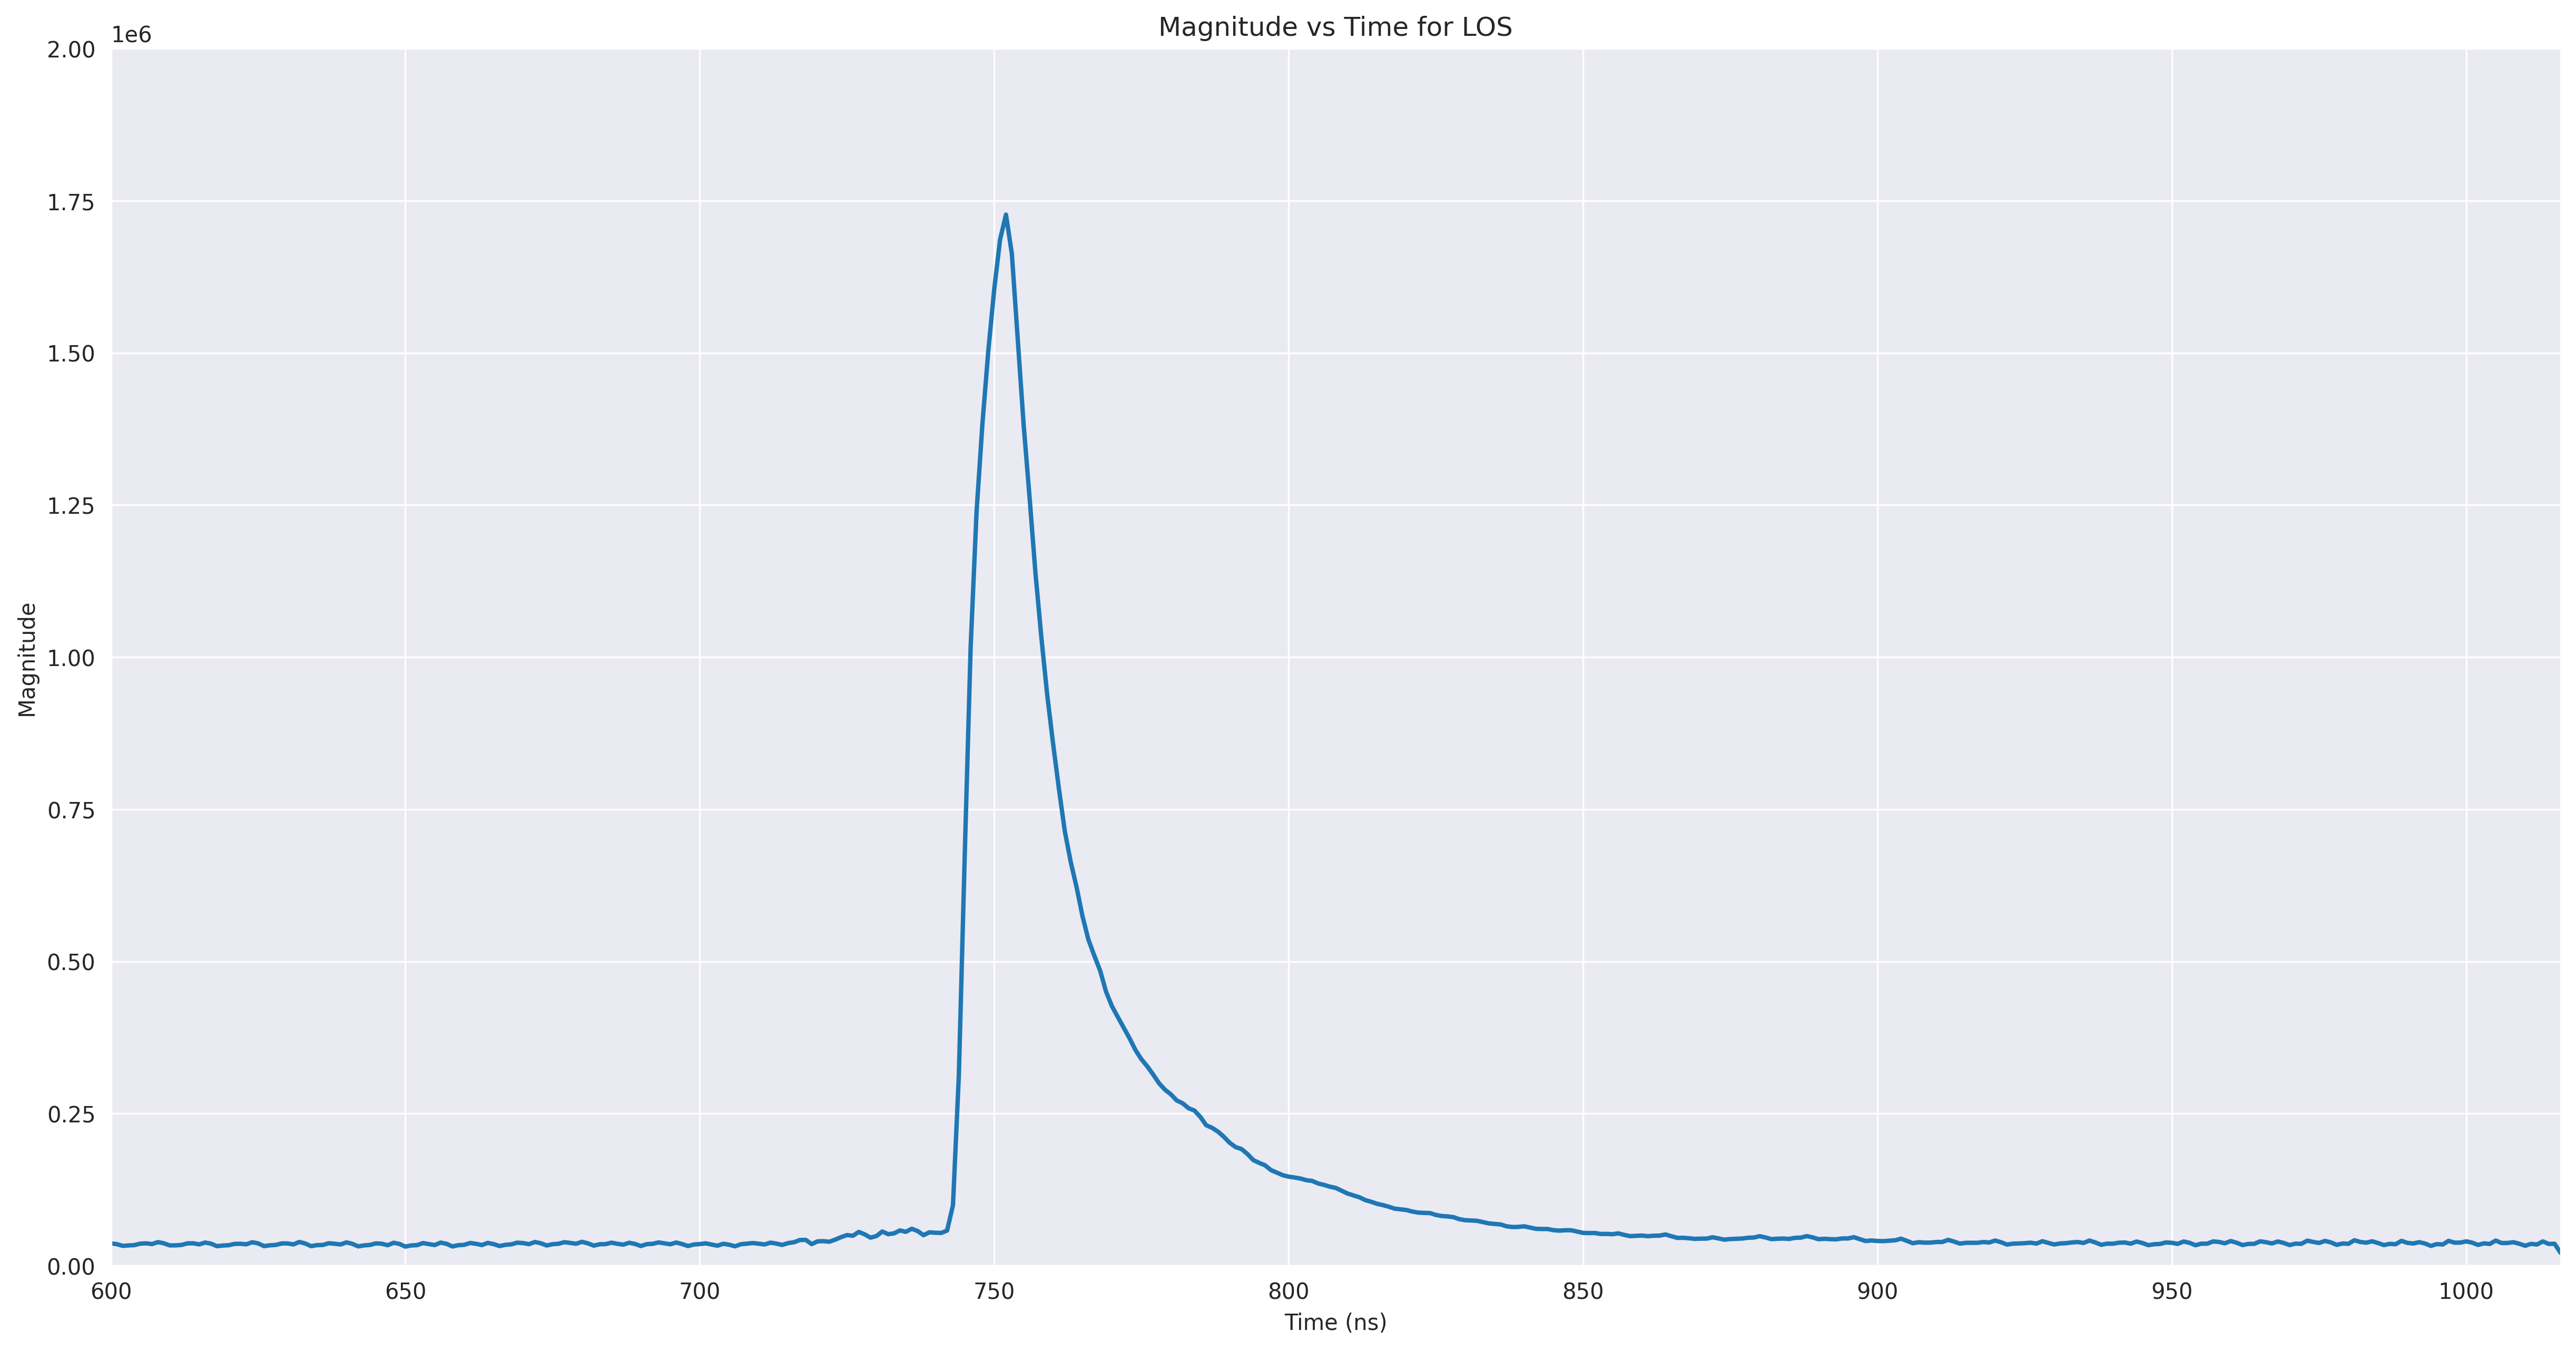
\includegraphics[width=0.4\textwidth]{preprocessing/LOS_Frequency_Graph.png}
	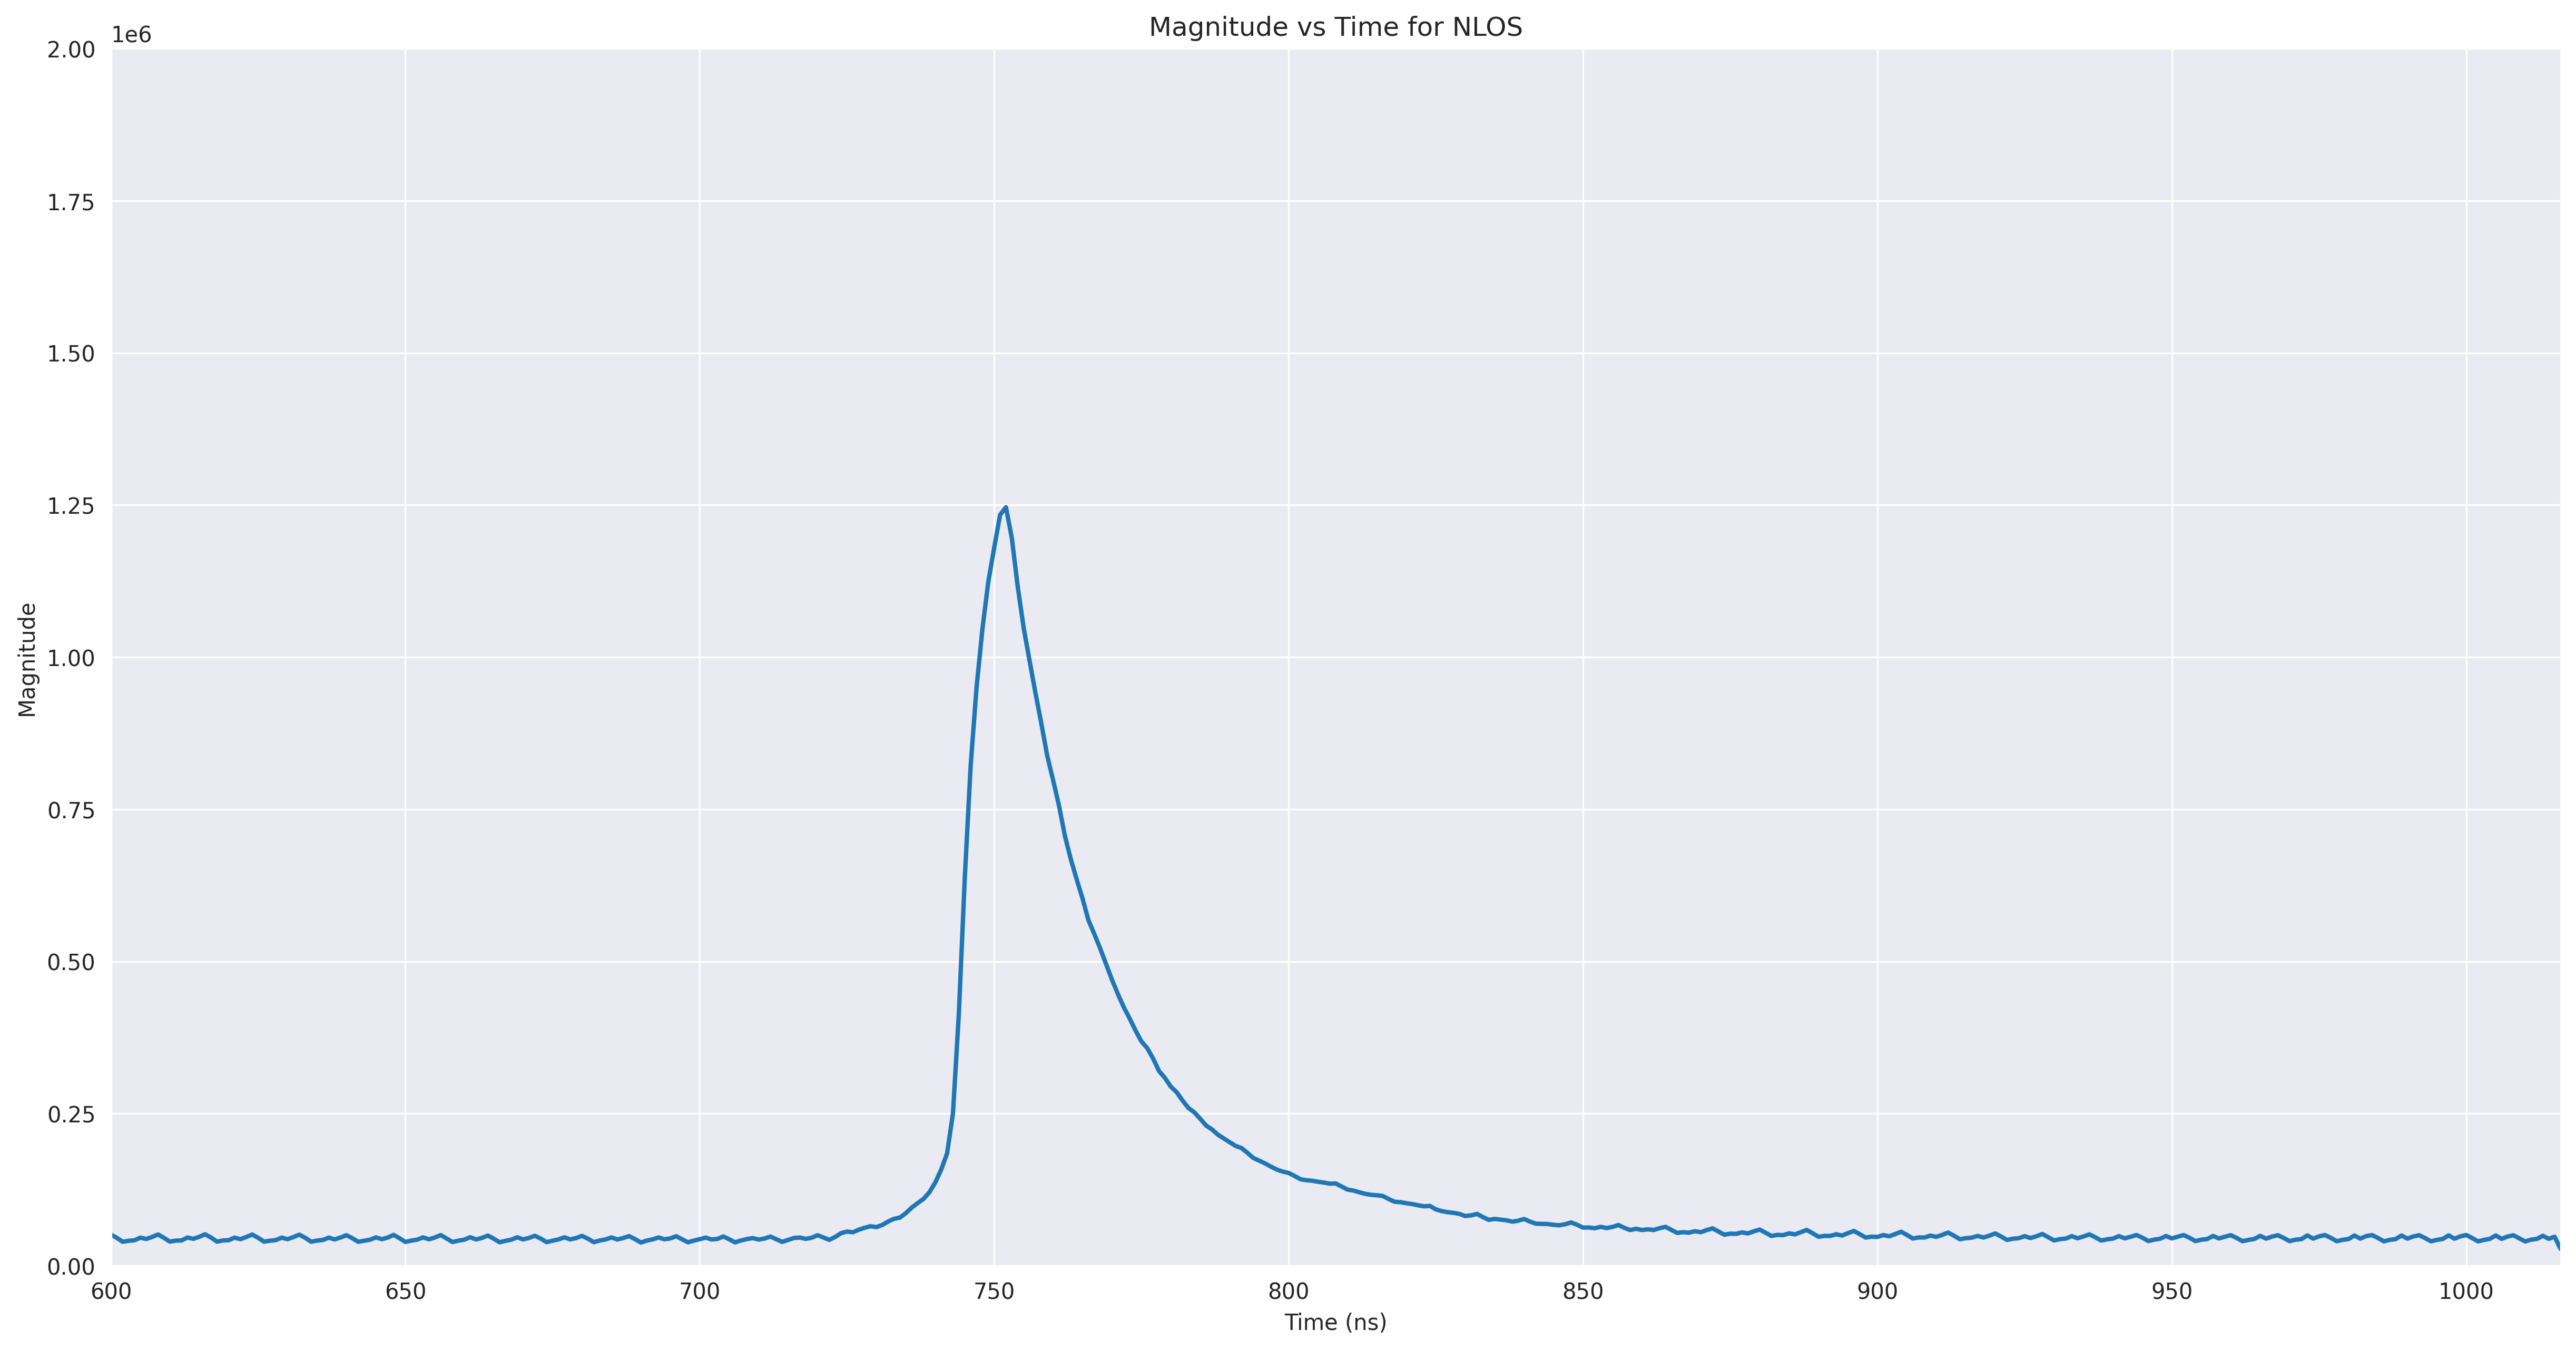
\includegraphics[width=0.4\textwidth]{preprocessing/NLOS_Frequency_Graph.png}
	\caption{Frequency Graph of LOS and NLOS}\label{fig:frequency_graph}
\end{figure}


Upon examining both LOS and NLOS \acrshort{cir} plots, several key observations emerge. Firstly, both plots display a prominent initial signal followed by a gradual decay over time. However, notable differences exist between the two scenarios. The LOS channel exhibits a stronger initial magnitude and a steeper decay compared to the NLOS channel, suggesting less signal distortion in the LOS scenario.

These observations have profound implications for machine learning models, particularly Convolutional Neural Networks (CNNs) and Multi-Layer Perceptrons (MLPs). While \acrshort{cir} data can serve as valuable input features for tasks like channel estimation or signal classification, raw \acrshort{cir} data may not be optimal for these models due to its complex nature.

To address this challenge, various data transformation techniques can be employed. The Discrete Fourier Transform (DFT) offers a method to convert \acrshort{cir} data into the frequency domain, enabling focused analysis on specific frequency bands relevant to the machine learning model. Additionally, the Wavelet Transform allows for comprehensive analysis of both time and frequency information embedded in the \acrshort{cir} data, potentially enhancing the model's understanding.

Moreover, techniques like Lucy-Richardson Deconvolution can be utilized to mitigate channel distortion in the \acrshort{cir} data, resulting in cleaner signals for the model to learn from. By integrating these data transformation techniques into the preprocessing stage, the effectiveness of CNNs and MLPs for tasks involving channel characterization can be significantly enhanced, ultimately leading to more robust and accurate communication systems.



\subsubsection{Frequency Graph of Wavelet Transformed LOS and NLOS}\label{frequency_graph_wavelet}

\begin{figure}[H] 
  \centering
  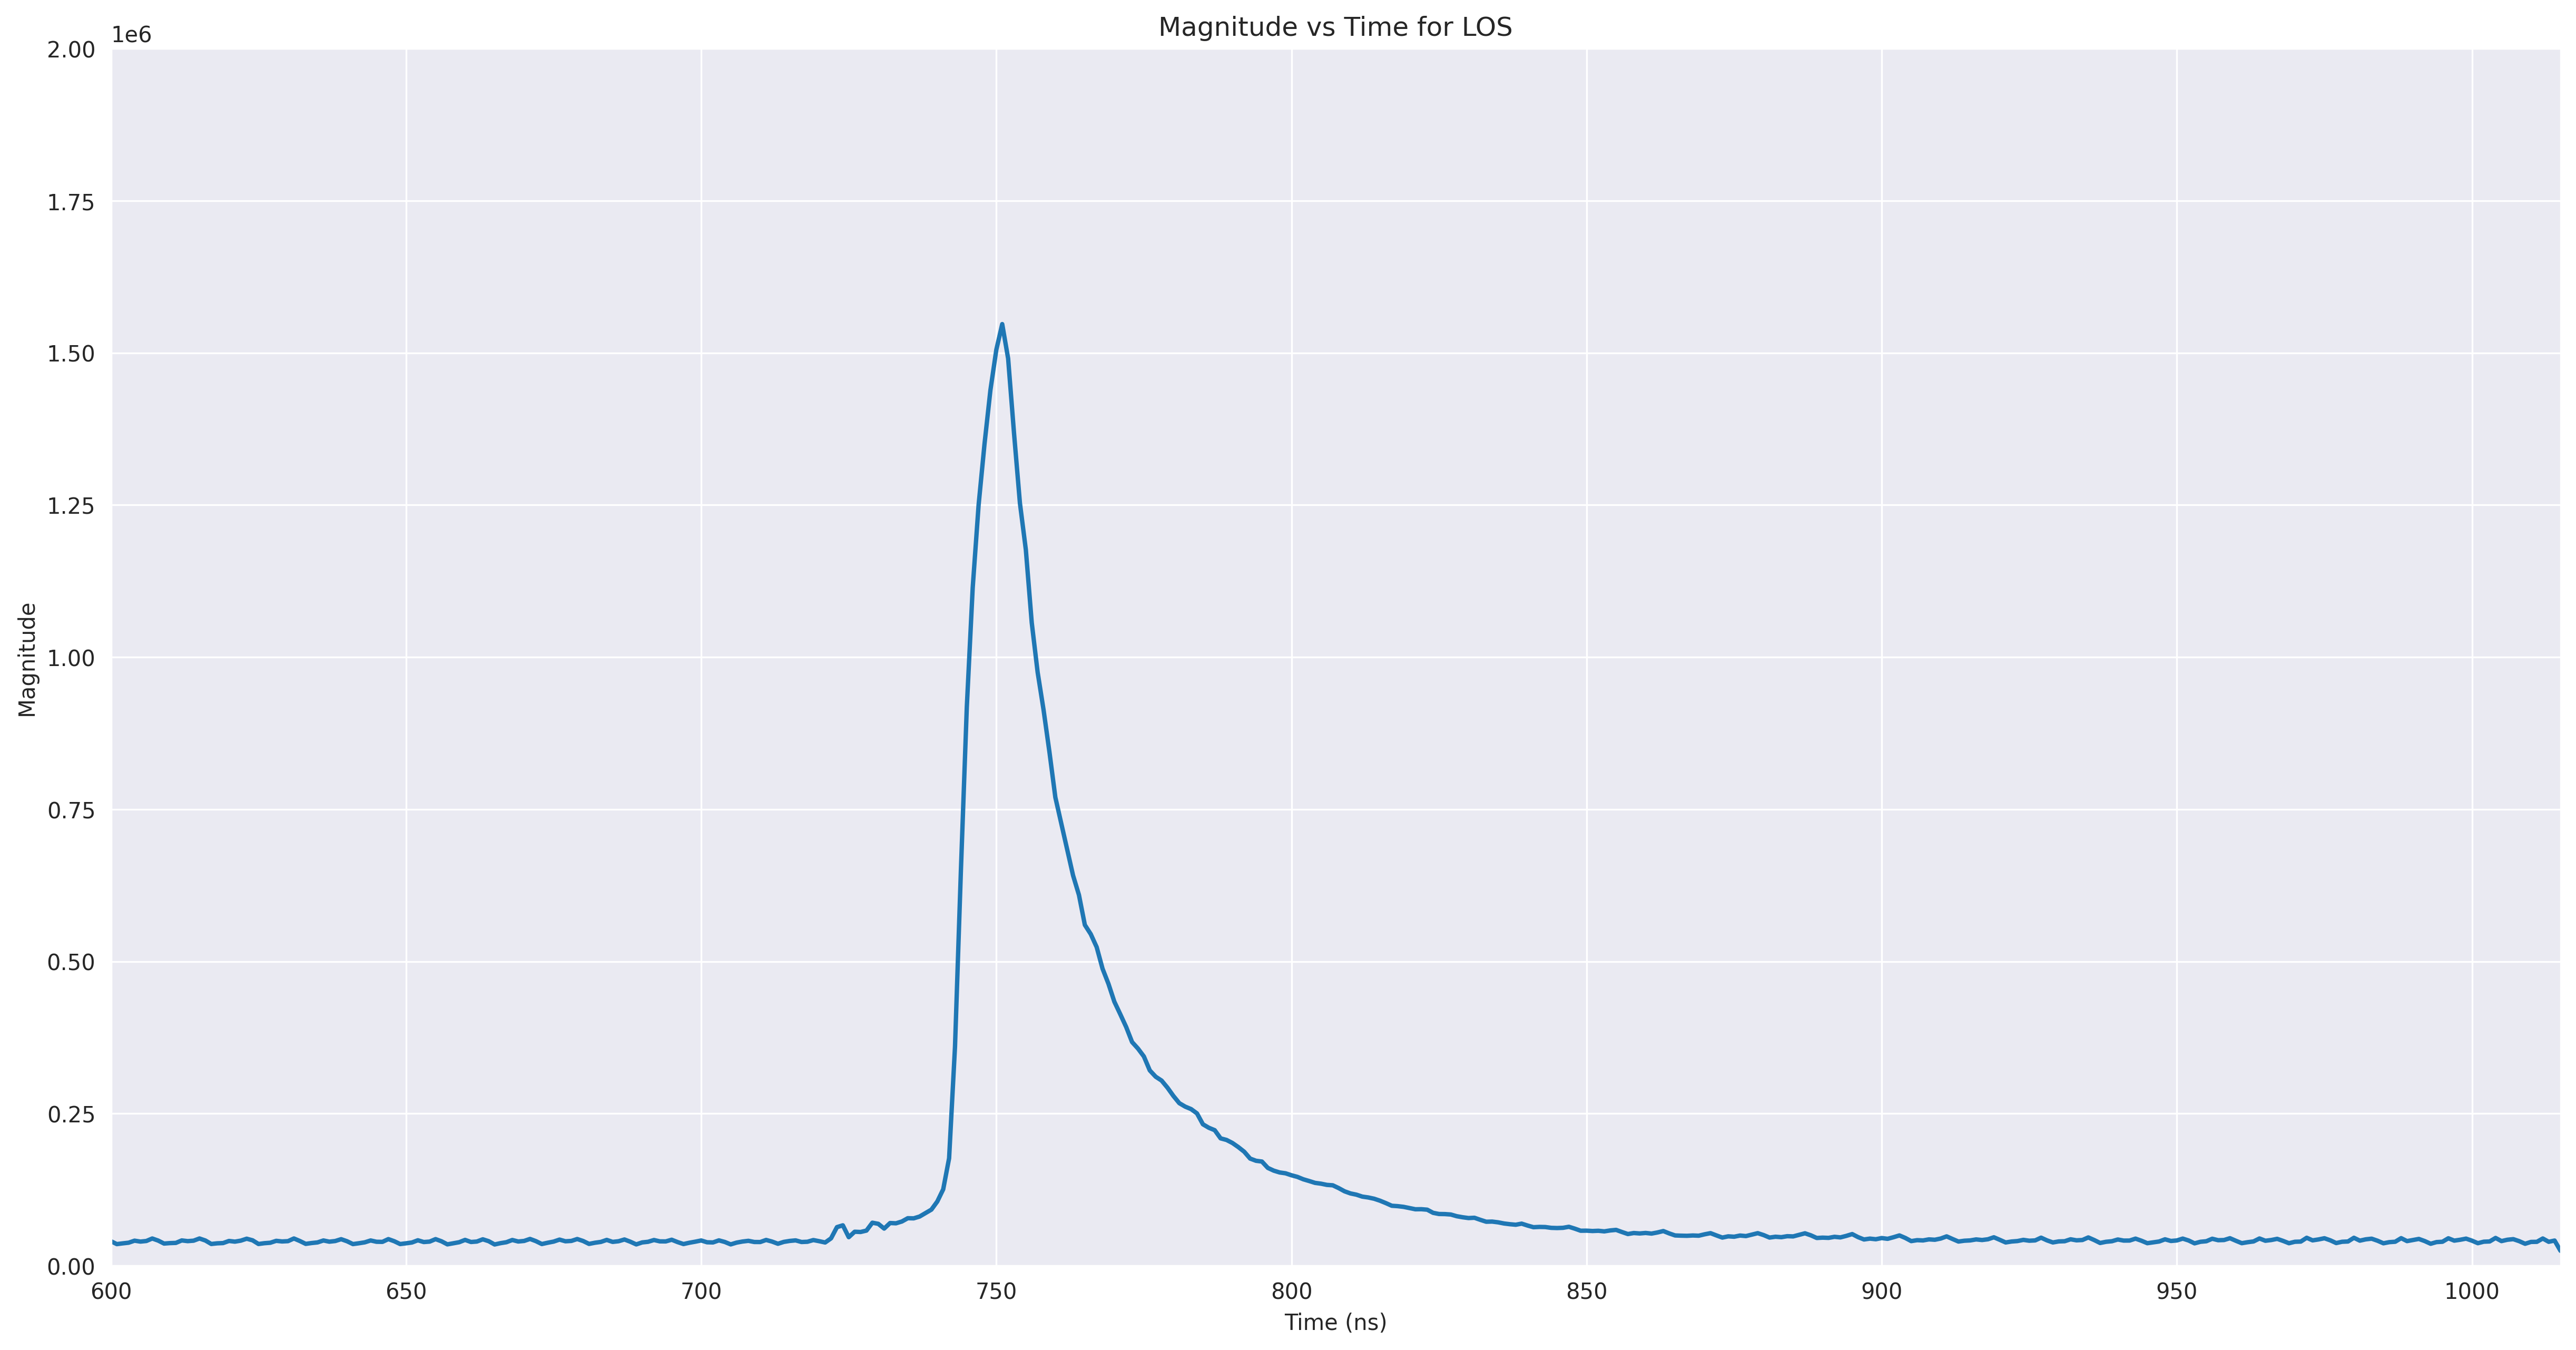
\includegraphics[width=0.4\textwidth]{preprocessing/Wavelet_Denoised_LOS_Frequency_Graph.png}
  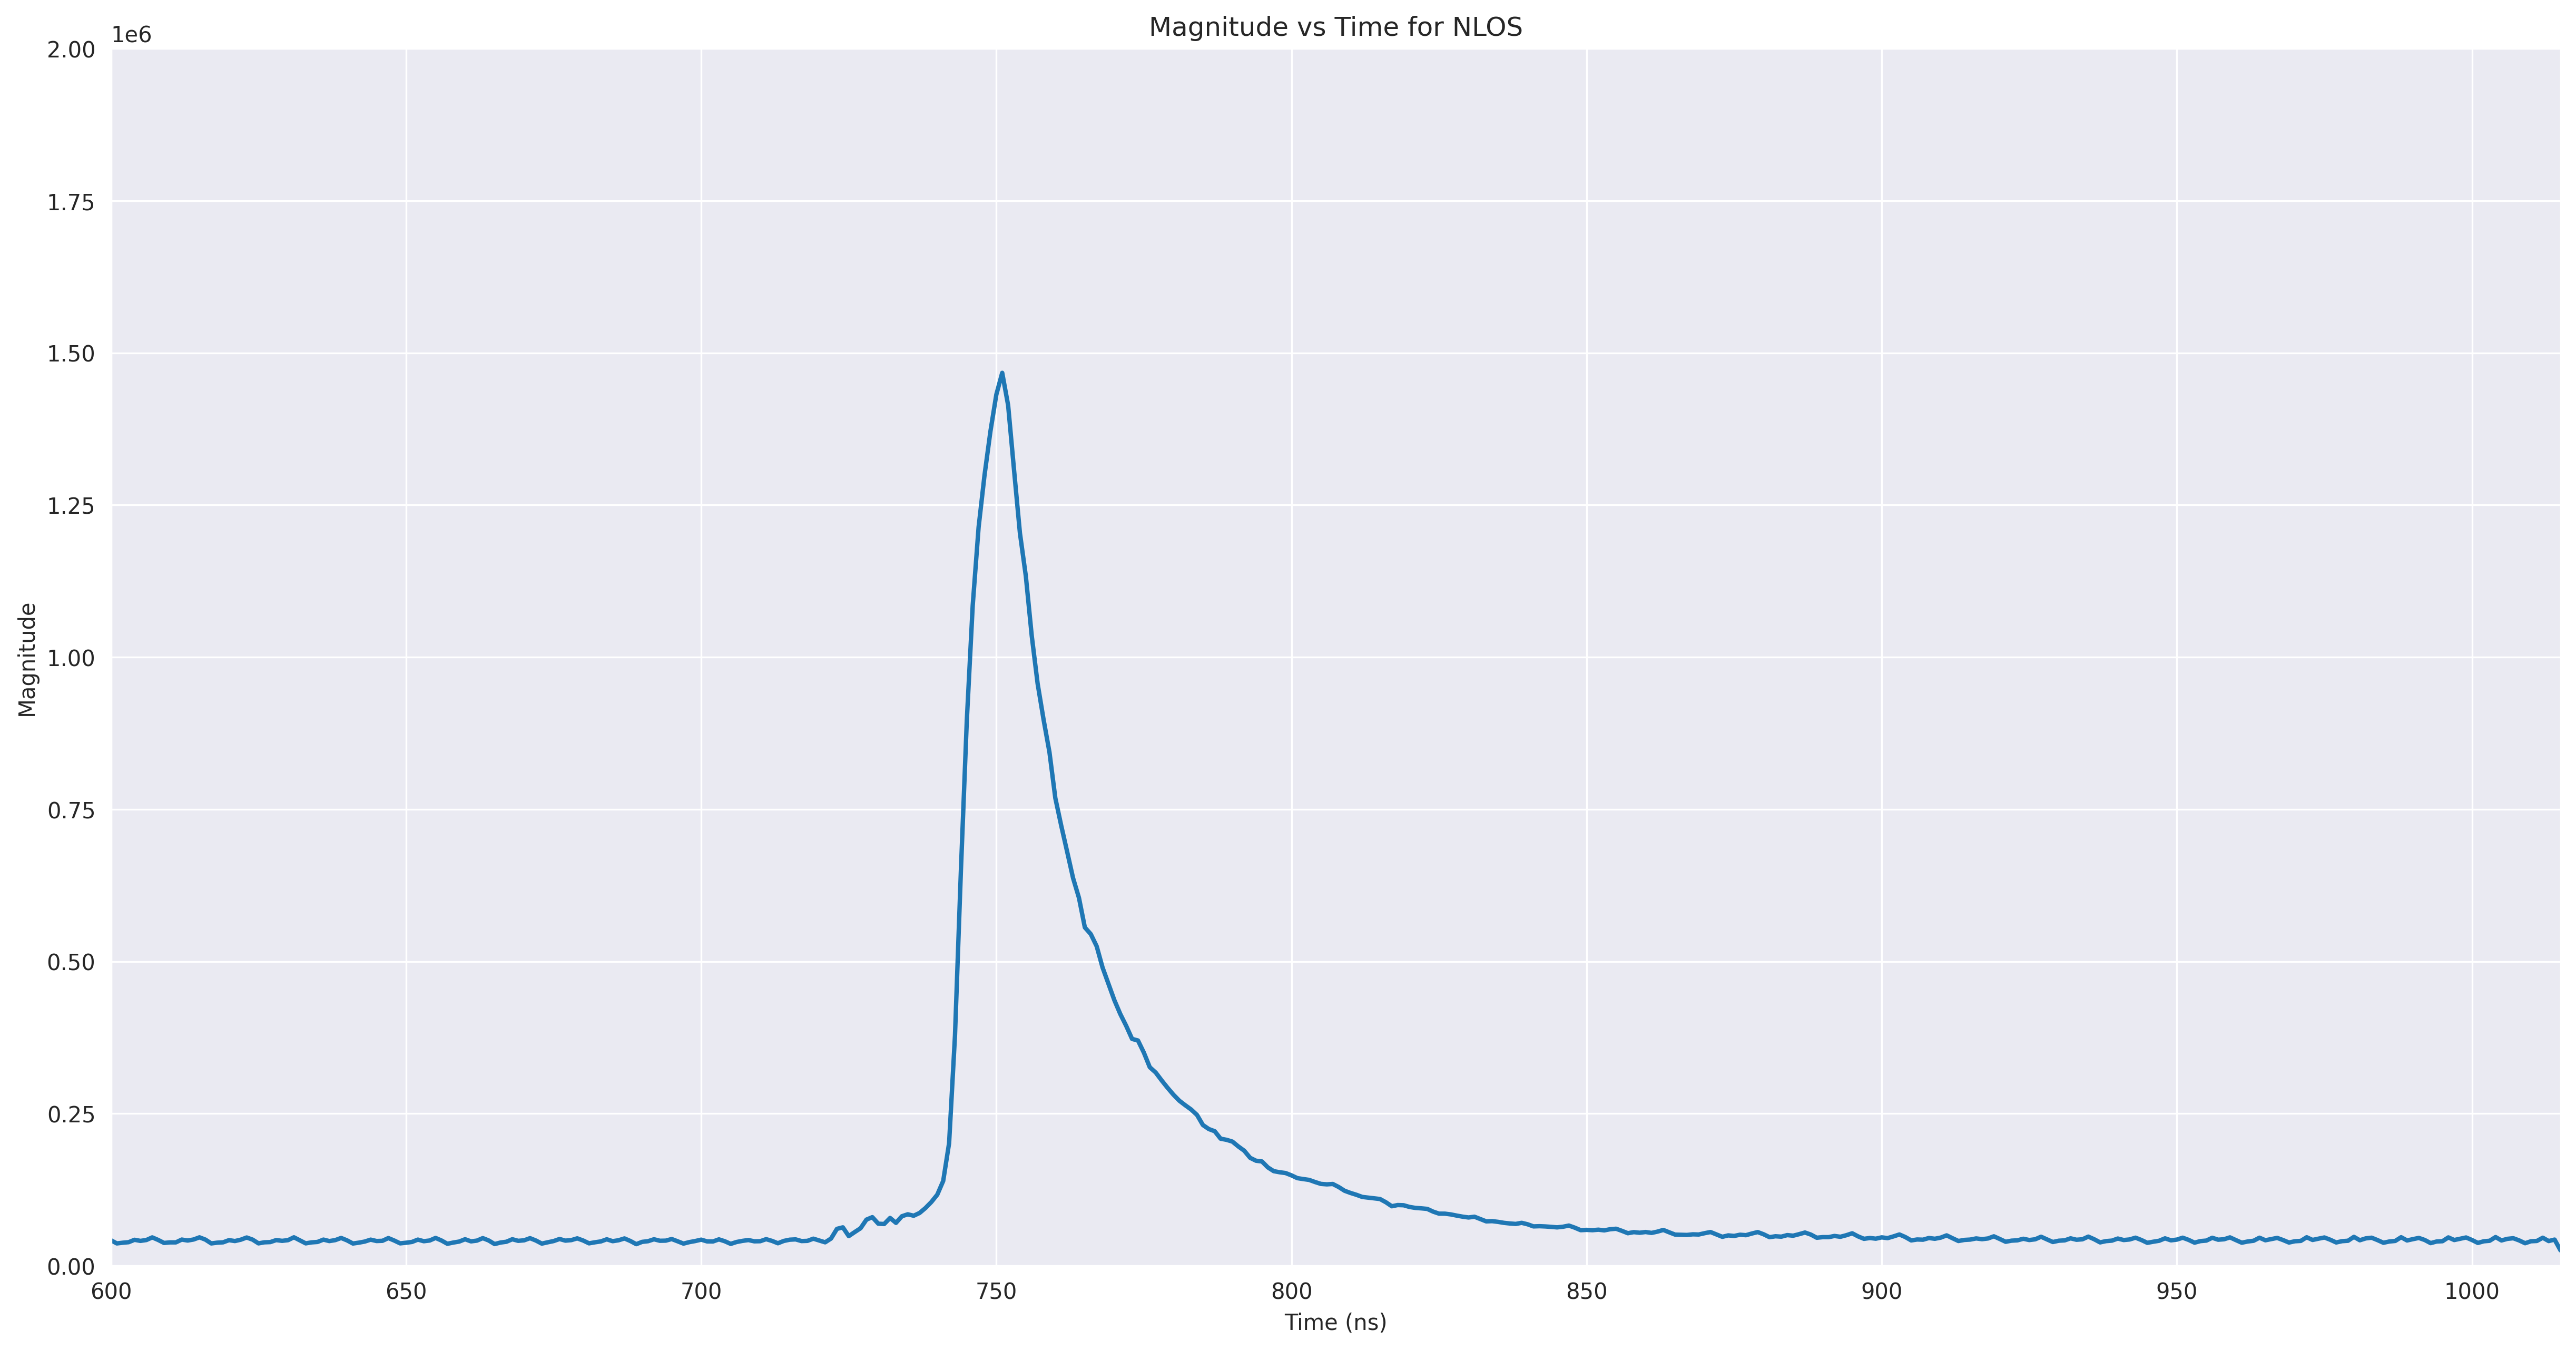
\includegraphics[width=0.4\textwidth]{preprocessing/Wavelet_Denoised_NLOS_Frequency_Graph.png}
  \caption{Frequency Graph of Wavelet Transformed LOS and NLOS}\label{fig:frequency_graph_wavelet}
\end{figure}

A comparison between the original and denoised NLOS \acrshort{cir} graphs reveals distinct differences. The original NLOS graph exhibits notable noise, characterized by fluctuations in magnitude, which can potentially obscure the underlying signal. In contrast, the denoised NLOS graph, resulting from successful wavelet denoising, presents a smoother profile, effectively removing noise while preserving the essential features of the signal.

Both the original and denoised LOS and NLOS \acrshort{cir} graphs demonstrate suitability for training Convolutional Neural Networks (CNNs) and Multi-Layer Perceptrons (MLPs). However, to enhance model performance, data pre-processing is recommended. 

Raw Channel Impulse Response (\acrshort{cir}) data may not be optimal for CNNs and MLPs due to its inherent complexity. Employing data transformation techniques such as the Discrete Fourier Transform (DFT) and Wavelet Transform can address this issue. The DFT allows focusing on specific frequency bands of interest, while the Wavelet Transform offers a more comprehensive time-frequency representation. Even denoised data can benefit from these transformations, potentially improving model performance significantly.

By integrating these pre-processing techniques into the workflow and transforming the \acrshort{cir} data (whether original or denoised) before training, CNNs and MLPs can effectively tackle tasks like channel estimation or signal classification, contributing to the development of robust communication systems.

\subsubsection{Frequency Graph of Lucy-Richardson Transformation LOS and NLOS}\label{frequency_graph_lr}

\begin{figure}[H] 
  \centering
  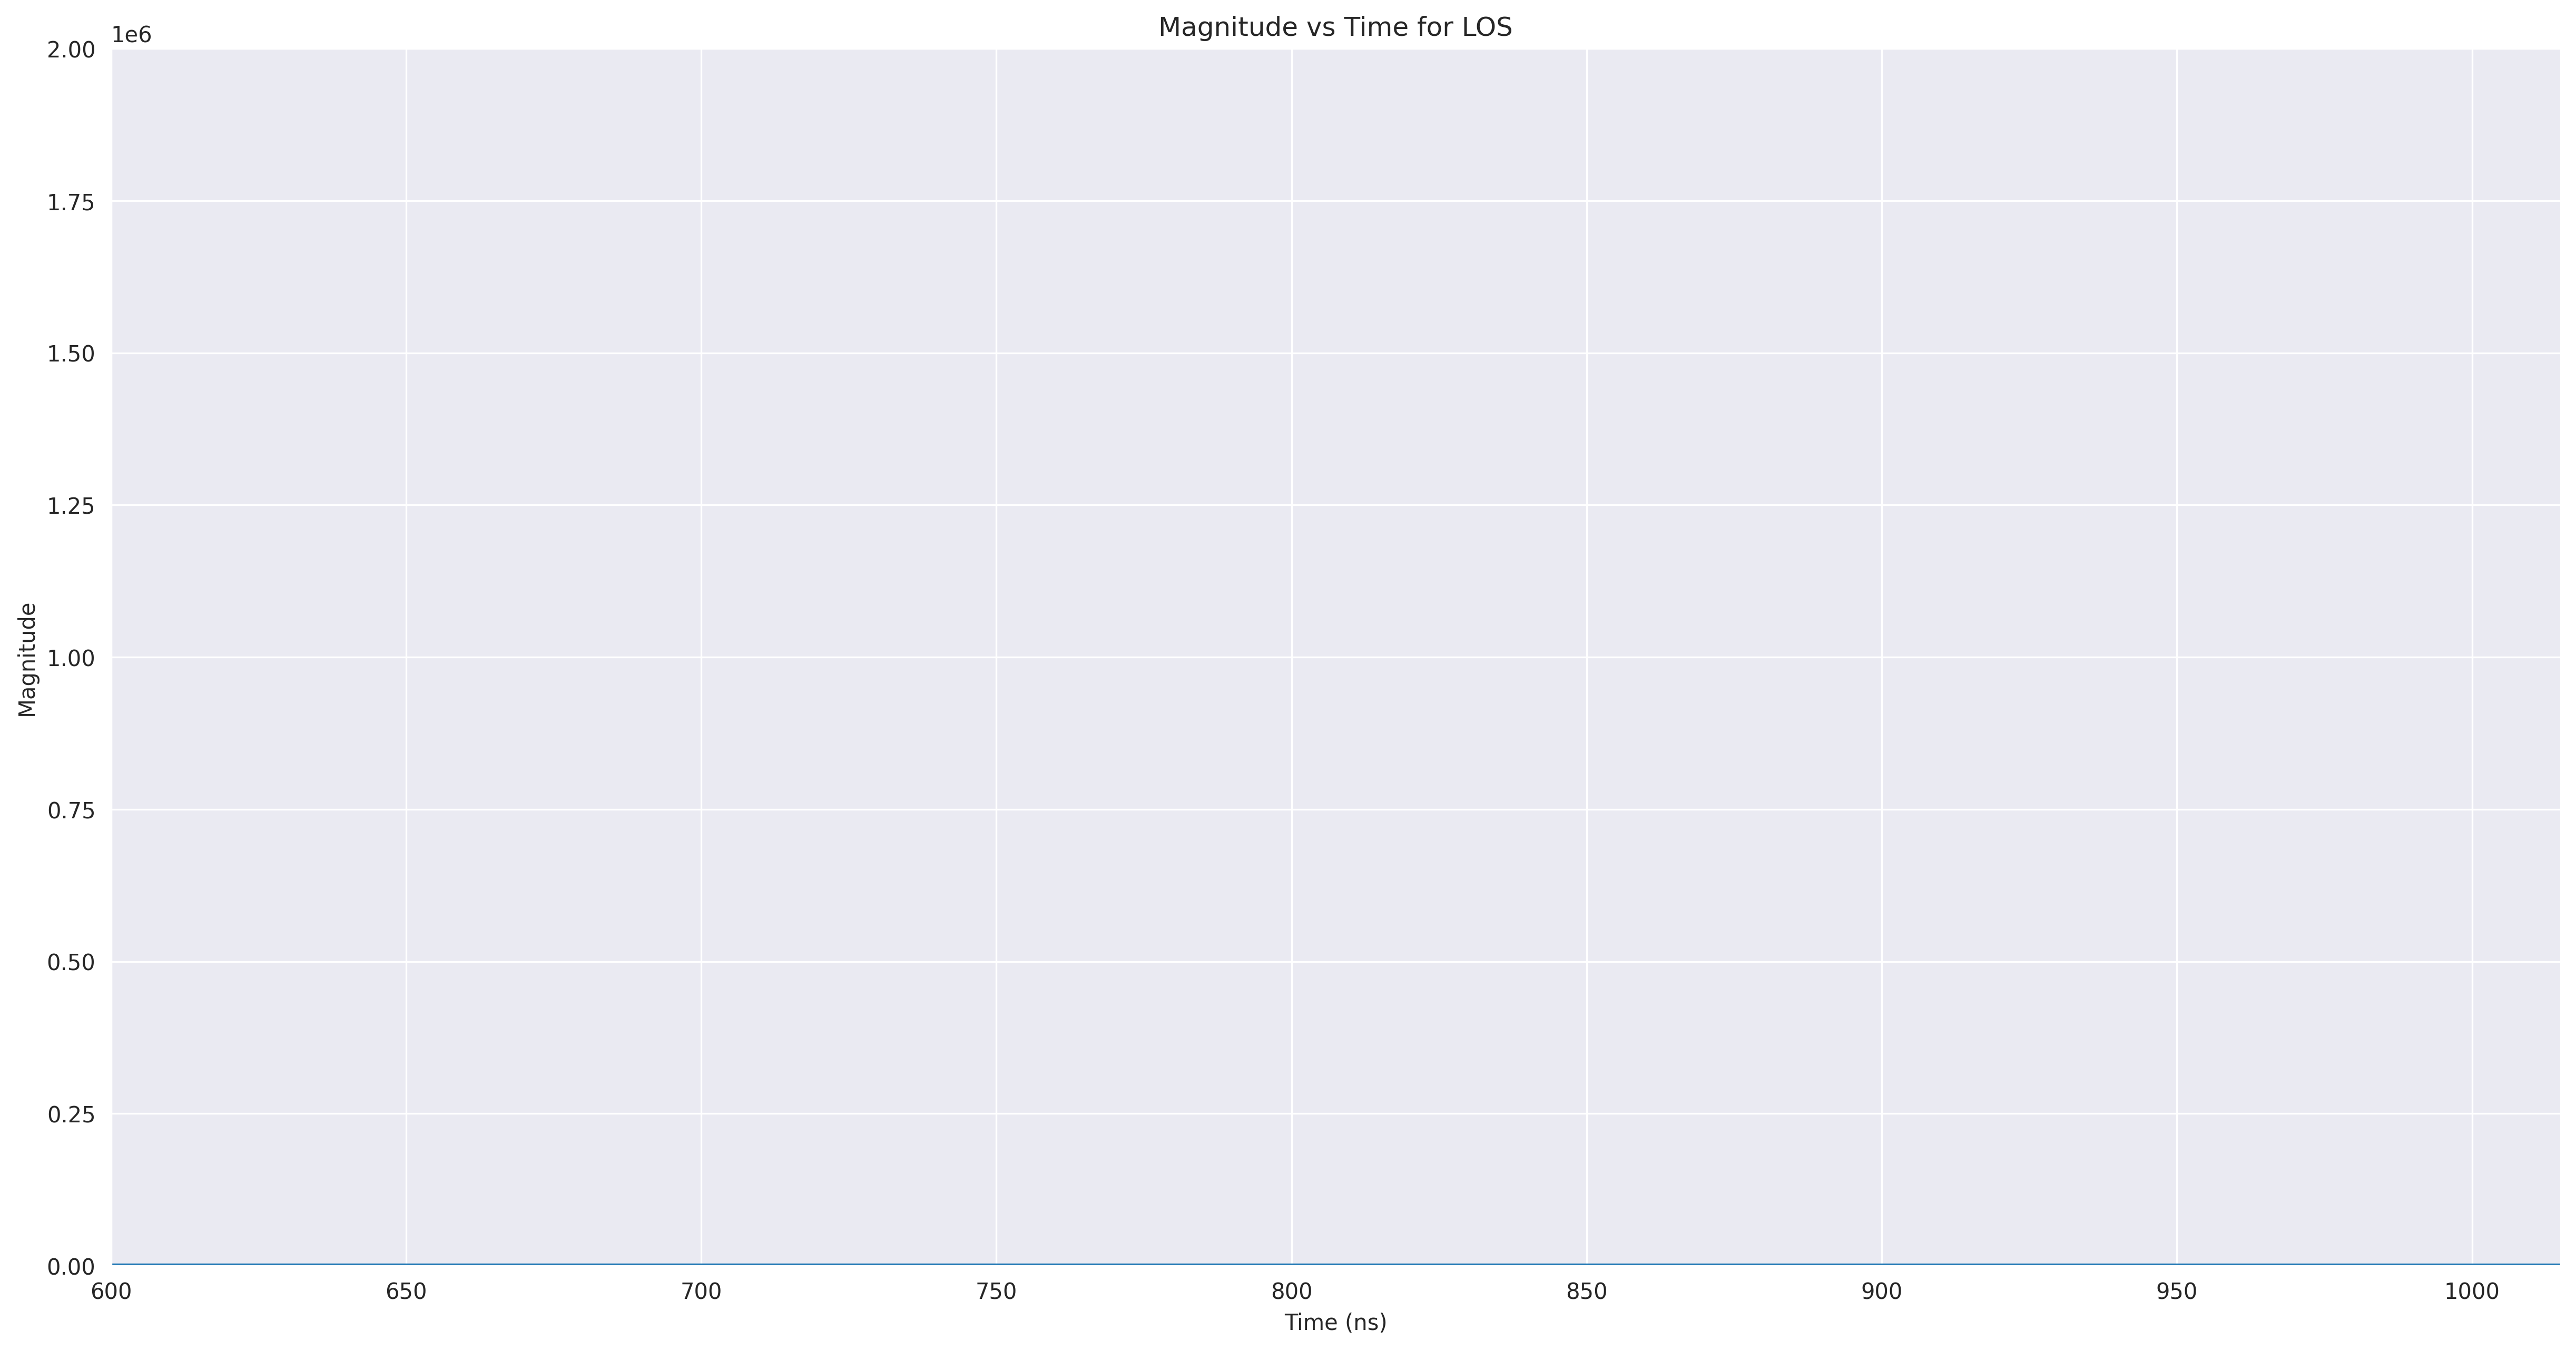
\includegraphics[width=0.4\textwidth]{preprocessing/lr_denoise_LOS.png}
  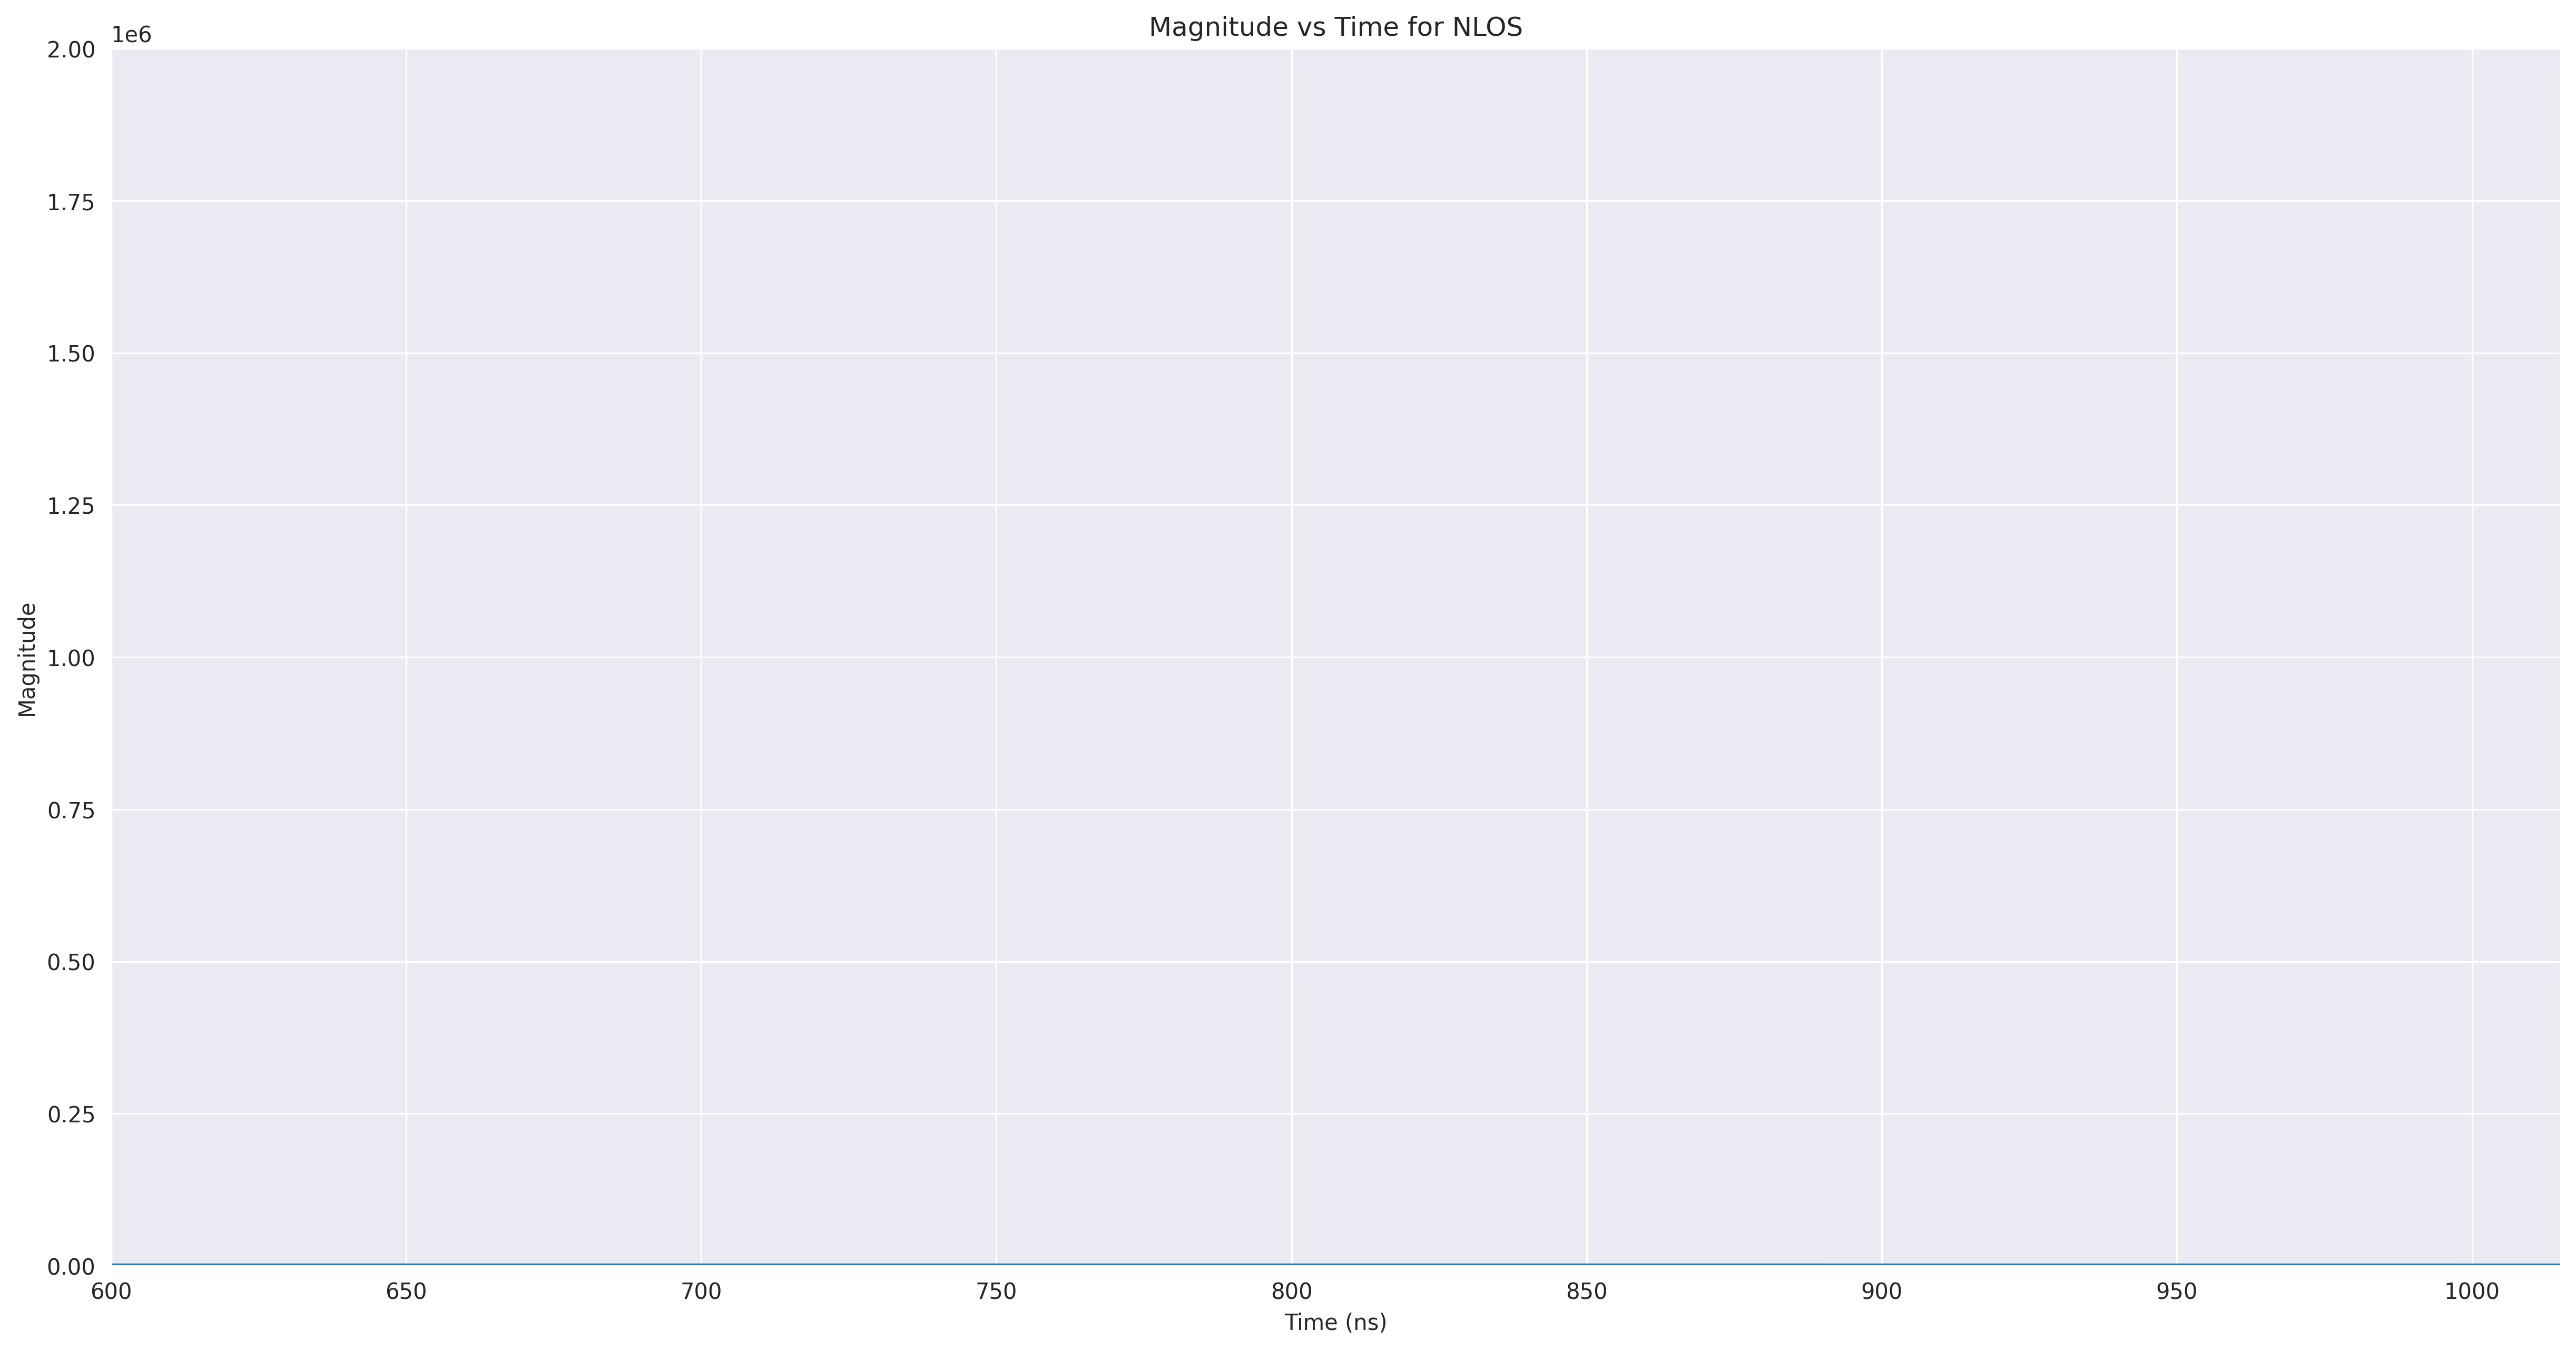
\includegraphics[width=0.4\textwidth]{preprocessing/lr_denoise_NLOS.png}
  \caption{Frequency Graph of Lucy-Richardson(Unscaled) LOS and NLOS}\label{fig:frequency_graph_lr}
\end{figure}

\begin{figure}[H] 
  \centering
  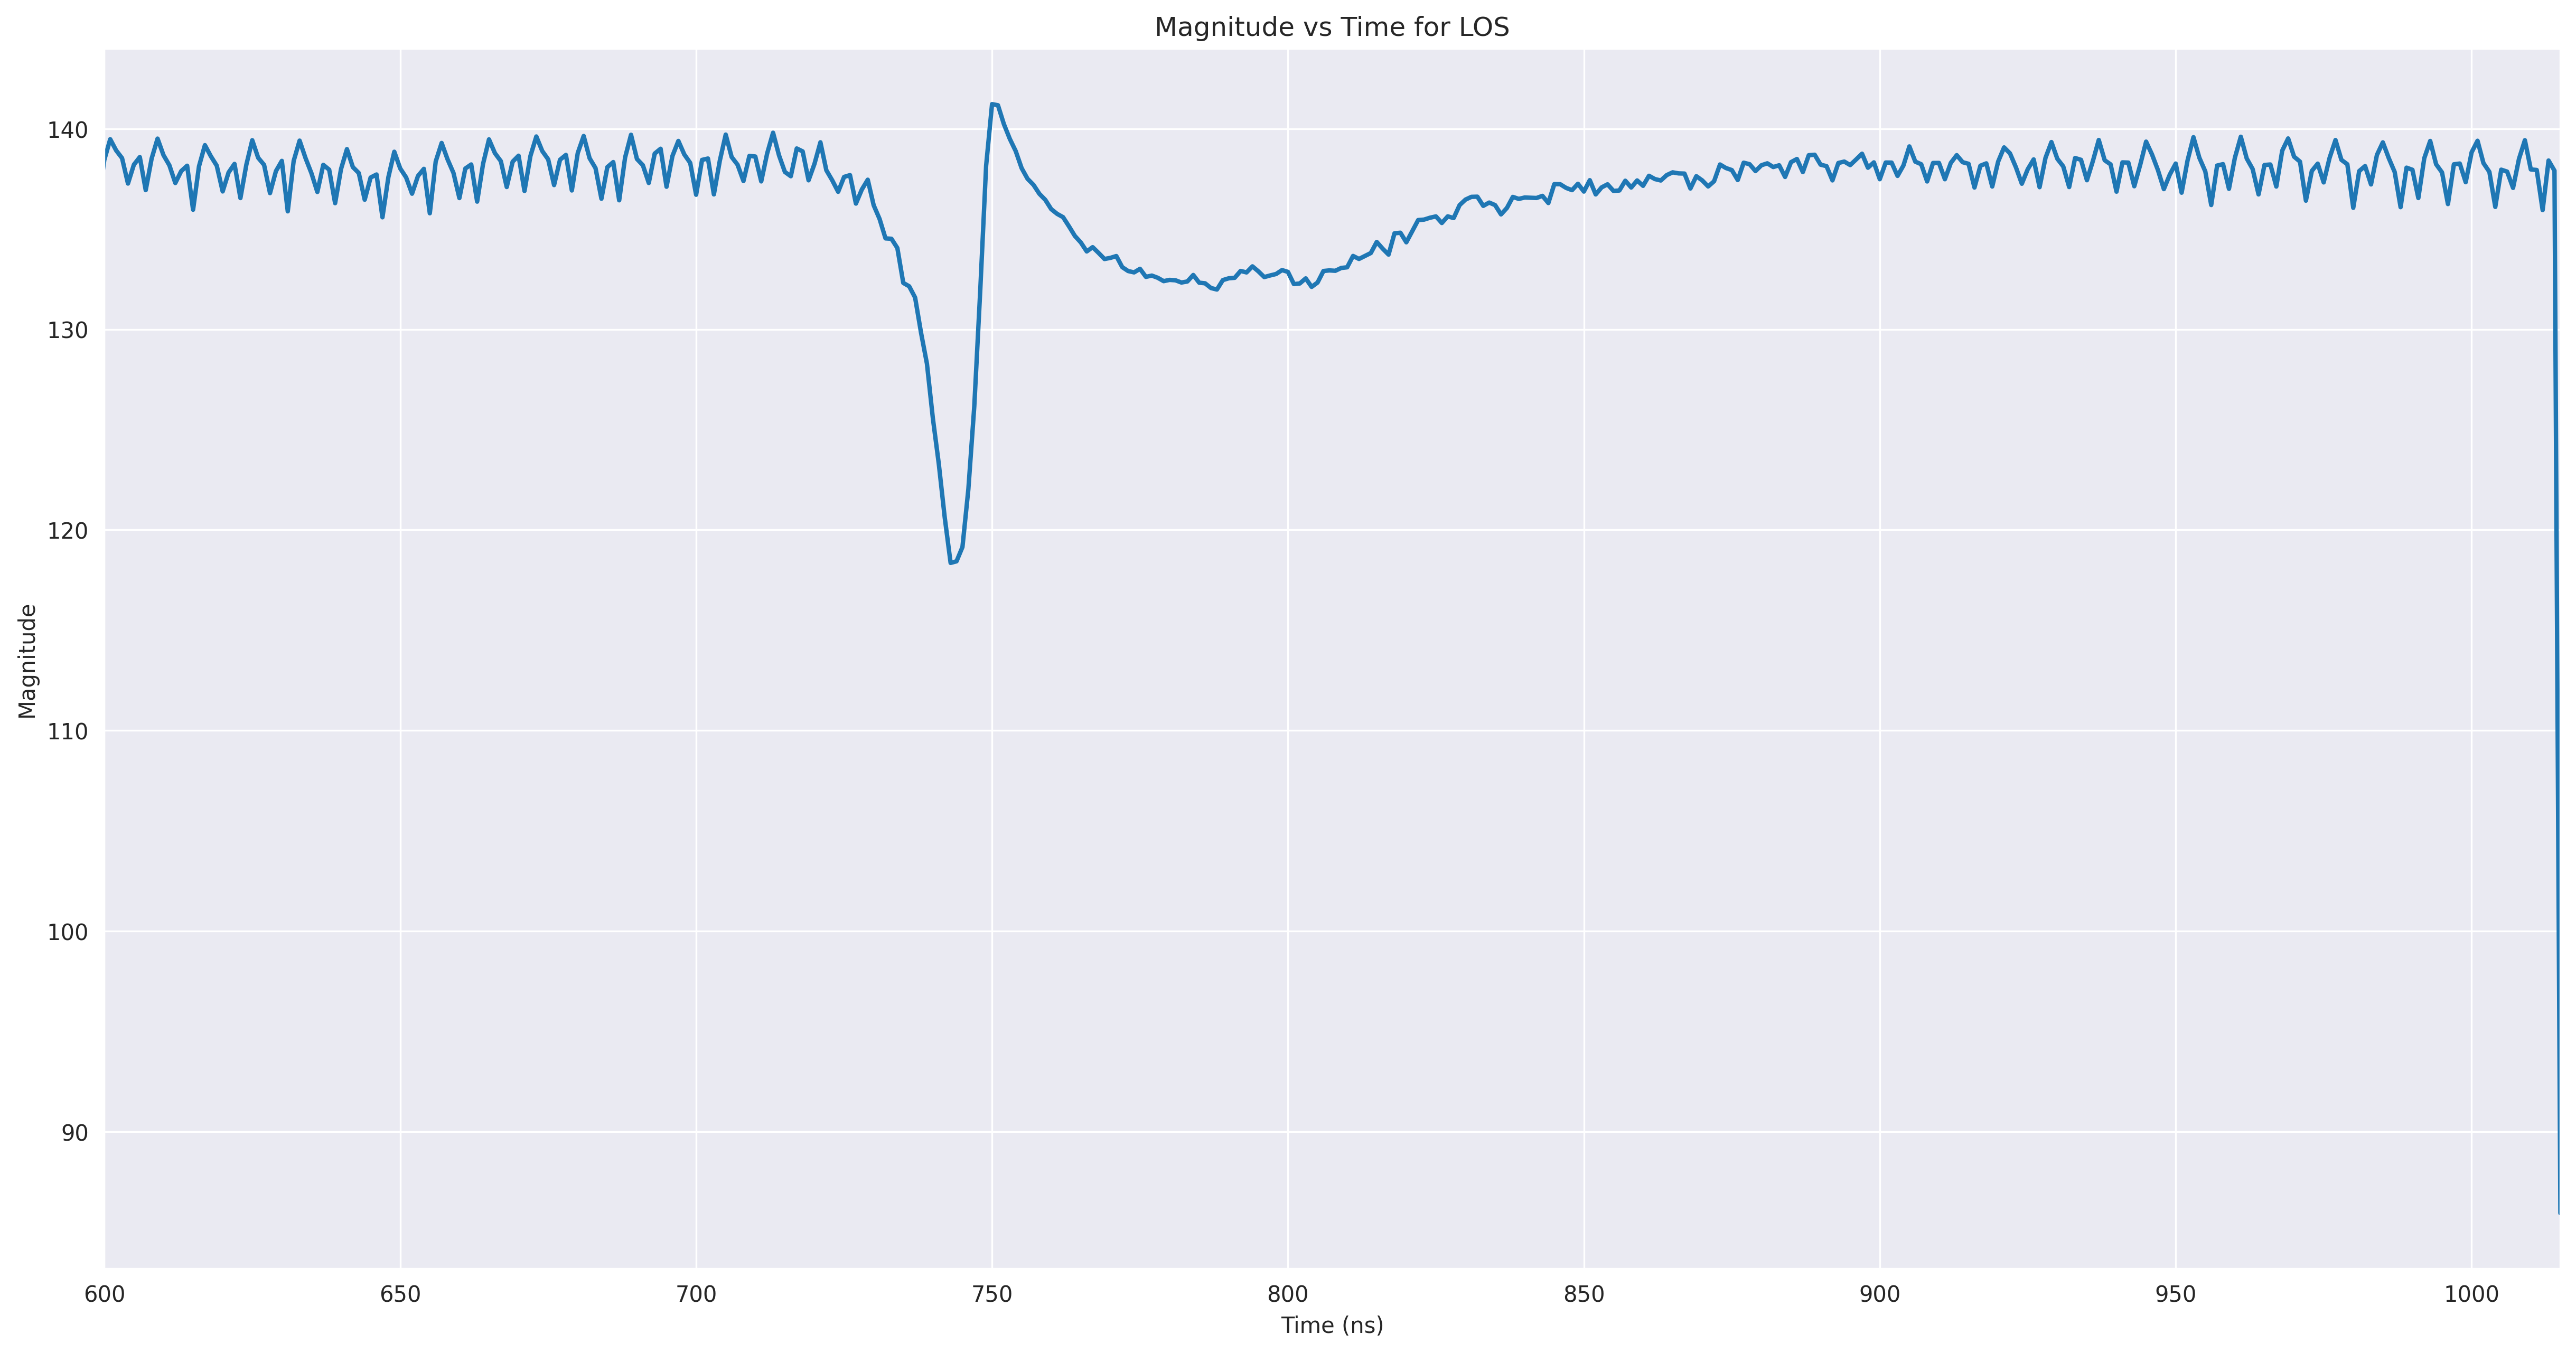
\includegraphics[width=0.4\textwidth]{preprocessing/lr_denoise_LOS_Scaled.png}
  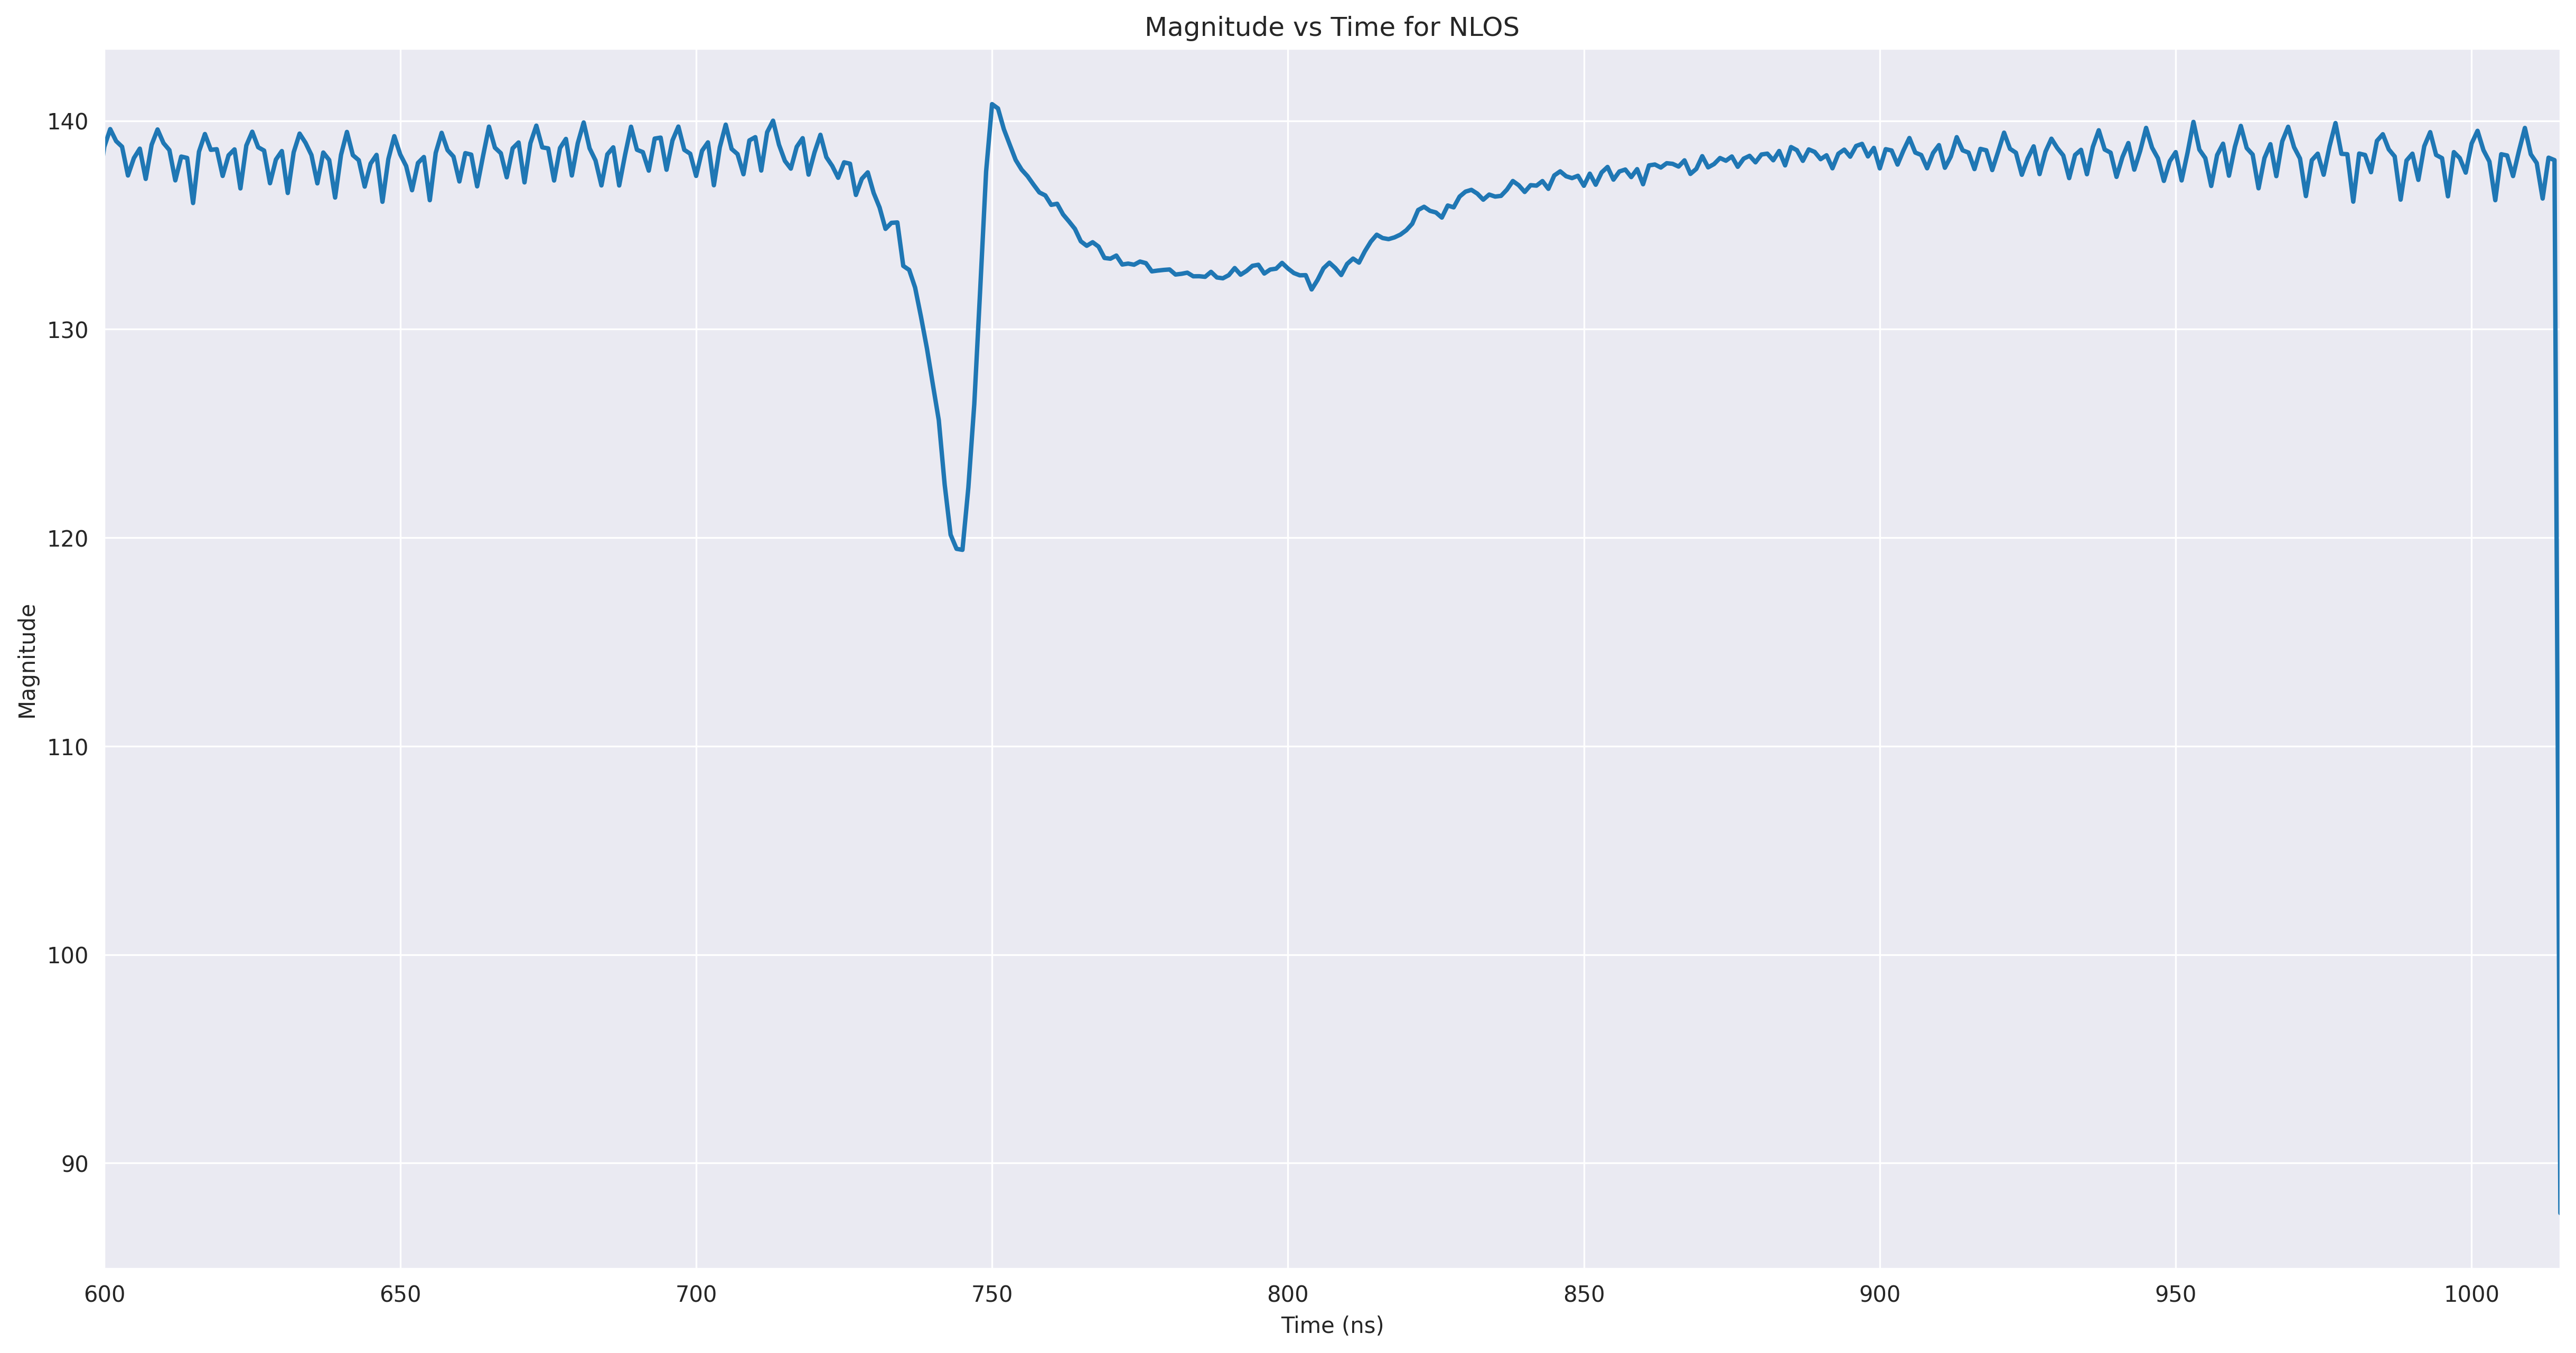
\includegraphics[width=0.4\textwidth]{preprocessing/lr_denoise_NLOS_Scaled.png}
  \caption{Frequency Graph of Lucy-Richardson(scaled) LOS and NLOS}\label{fig:frequency_graph_lr_scaled}
\end{figure}

% MENTION WHY THIS WASNT USED IN TRAINING
% added this can help fact check - jwisgay %
% The frequency graphs of the Lucy-Richardson scaled \gls{los} and \gls{nlos} \acrshort{cir}s offer a profound insight into the spectral characteristics of communication channels. The application of the Lucy-Richardson deconvolution technique transforms the CIR data, mitigating the distortive effects of the channel and revealing the intrinsic frequency properties of the LOS and NLOS scenarios. The resulting frequency domain representation showcases a refined contrast between the LOS and NLOS conditions, highlighting variations that are essential for robust model differentiation.

% This enhanced frequency domain data is particularly vital for the training of sophisticated machine learning models like CNNs and MLPs. These models thrive on detailed and variegated datasets, and the Lucy-Richardson scaling provides a frequency-based complexity that enriches the input data. It allows the models to discern intricate patterns and to generalize effectively, leading to more nuanced signal classification and channel estimation tasks.

% By incorporating Lucy-Richardson scaled frequency data into the training process, we can significantly elevate the performance of CNNs and MLPs. Such a nuanced spectral perspective equips these models to capture the essence of the signal propagation characteristics, distinguishing LOS from NLOS with higher accuracy. Ultimately, this paves the way for more resilient communication systems that can navigate and adapt to complex environmental dynamics.

% REFINED ver @ jwisgay, is this better? %
Lucy-Richardson deconvolution significantly refines \acrshort{cir} data for LOS and NLOS scenarios, providing enriched frequency domain representations that are key for robust differentiation by advanced machine learning models such as CNNs and MLPs. This technique reveals the deeper spectral characteristics of communication channels, diminishing distortive effects and allowing for the extraction of intricate patterns, thus facilitating more accurate signal classification and channel estimation tasks. Incorporating such scaled frequency data elevates model performance, capturing essential signal propagation nuances to distinguish LOS from NLOS scenarios more precisely, fostering the development of adaptive, resilient communication systems.

However, the practical application of Lucy-Richardson scaling is complex. Its computationally intensive nature could impose significant demands on resources, particularly for larger datasets, leading to prolonged training times. This complexity, coupled with the potential for overfitting and the introduction of artifacts or loss of crucial time-domain information, requires careful deliberation. Additionally, this sophisticated signal processing necessitates specialized knowledge and tools, presenting a barrier to its routine implementation in training protocols. While the benefits of incorporating this scaled data are clear, the constraints of computational cost, model complexity, and domain-specific suitability must be judiciously weighed to determine the technique's feasibility in enhancing machine learning frameworks.
% end of check - help check jwisgay %

\subsubsection{Discrete Fourier Transform}\label{dft_visual}

\begin{figure}[H] 
  \centering
  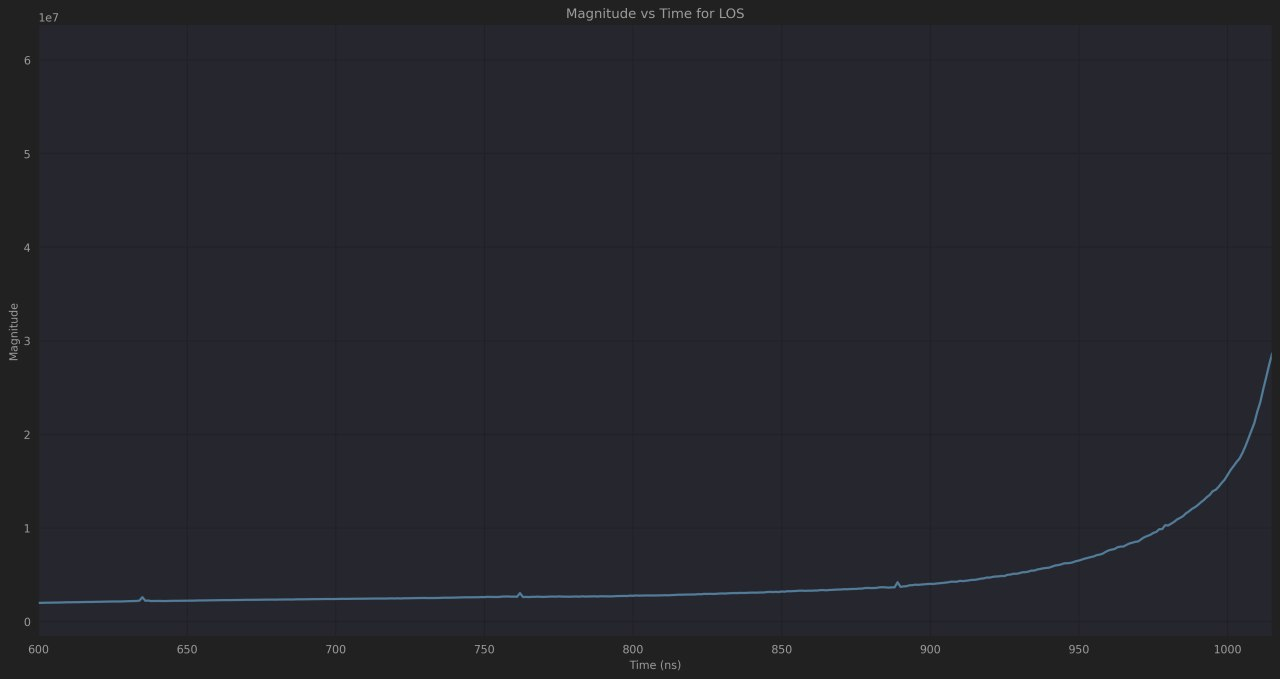
\includegraphics[width=1\textwidth]{preprocessing/DFT_LOS.jpg}
  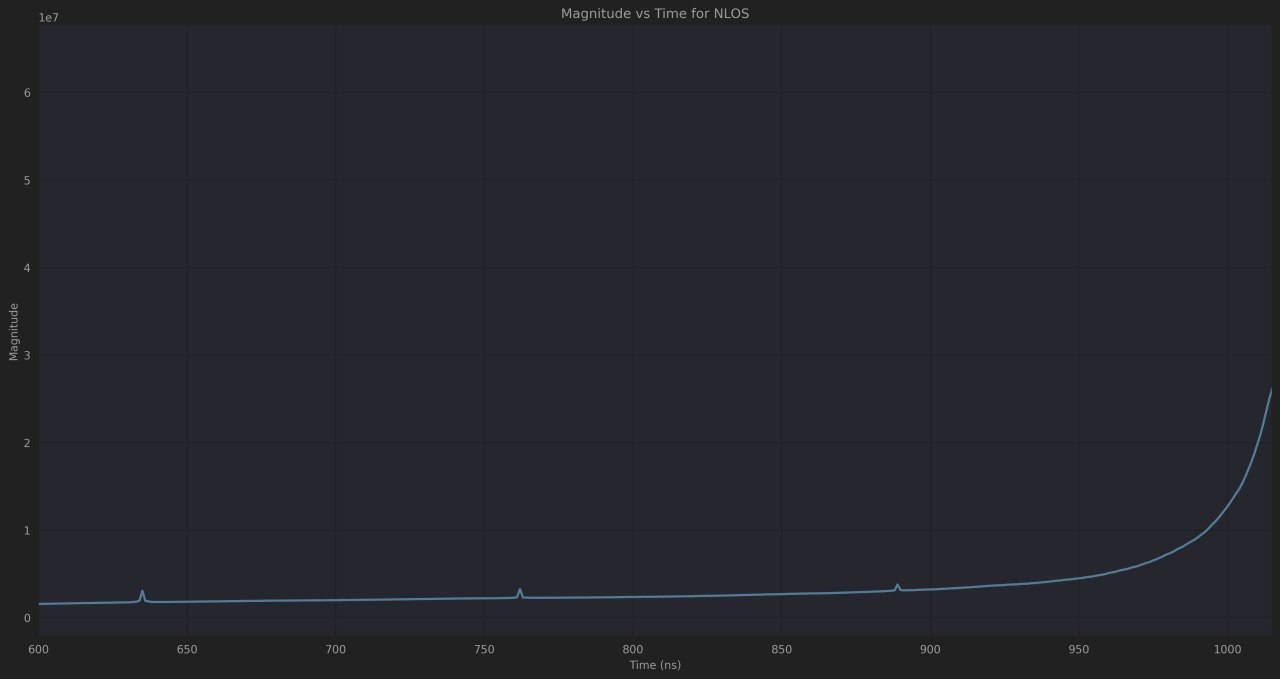
\includegraphics[width=1\textwidth]{preprocessing/DFT_NLOS.jpg}
  \caption{Frequency Graph of Discrete Fourier Transformed \acrshort{cir} values (LOS and NLOS)}\label{fig:frequency_graph_dft}
\end{figure}

The figures display the outcome of applying the Discrete Fourier Transform (DFT) to the original \acrshort{cir} data. DFT converts the signal from the time domain (original graph) to the frequency domain (DFT graph), revealing where the signal energy lies across different frequencies.

The original \acrshort{cir} data shows signal strength over time, while the DFT plots uncover which frequencies carry the most significant signal power. This preprocessing step is vital for CNN and MLP models because they excel at identifying patterns within data. By presenting \acrshort{cir} data in the frequency domain, DFT highlights these patterns, simplifying the learning process for models and potentially enhancing performance in tasks such as signal (\gls{los} / \gls{nlos}) classification.

\subsubsection{Signal to Noise Ratio}\label{snr_visual}

\begin{figure}[H]
	\centering
	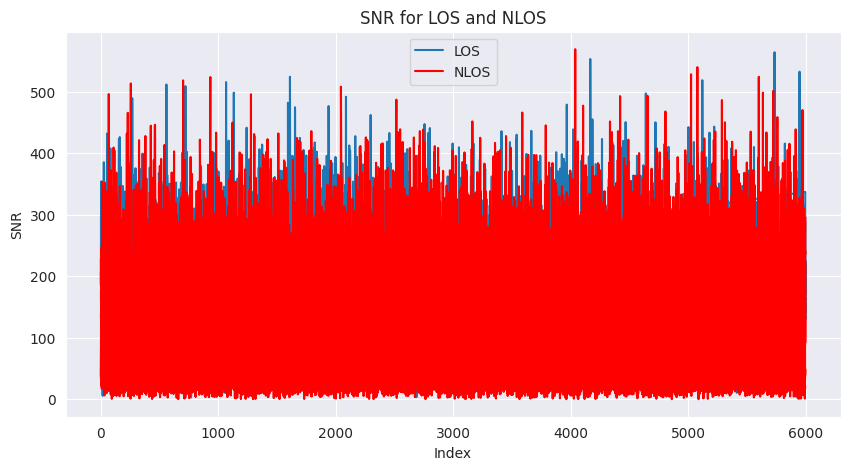
\includegraphics[width=1\textwidth]{preprocessing/SNR} % Include the figure
	\caption{Signal to Noise Ratio}\label{fig:snr}
\end{figure}

This graph displays the Signal-to-Noise Ratio (SNR) for both LOS (Line-of-Sight) and NLOS (Non-Line-of-Sight) scenarios.  A higher SNR indicates a stronger signal relative to noise. The graph confirms a stronger signal in the LOS case.

While the SNR itself is informative for channel classification or quality estimation, the raw SNR graph might not be ideal for training models like CNNs and MLPs. These models typically prefer raw data (like the original \acrshort{cir} data) to learn features themselves. So, the original \acrshort{cir} data might be more suitable for training compared to just the extracted SNR value.

%%%%%%%%%%%%%%%%%%%%%%%%%%%%%%%%%%%%%%%%%%%%%%%%%
% CNN Visualisation 
%%%%%%%%%%%%%%%%%%%%%%%%%%%%%%%%%%%%%%%%%%%%%%%%%

\subsection{Convolution Neural Network}\label{cnn_visual}

\begin{figure}[H] 
  \centering
  \includegraphics[width=1\textwidth]{cnn/CNN_Confusion_Matrix.png}
  \caption{CNN Confusion Matrix}\label{fig:cnn_confusion_matrix}
\end{figure}

% help check pl0x - jwisgay %
% ben ben help check pl0x too %
The presented confusion matrix reflects the CNN's classification accuracy without employing DFT preprocessing. With 3808 true negatives and 3441 true positives, the model demonstrates a commendable ability to identify both classes. However, the presence of 384 false positives and 767 false negatives highlights areas where the model's predictive precision can still be enhanced. The results suggest that while the CNN is quite capable of discerning between the classes, integrating strategies to improve its sensitivity and specificity potentially through preprocessing techniques like DFT or model tuning could further refine its performance.


\begin{figure}[H] 
  \centering
  \includegraphics[width=1\textwidth]{cnn/CNN_Learning_Curve.png}
  \caption{CNN Learning Curve}\label{fig:cnn_learning_curve}
\end{figure}

% help check pl0x - jwisgay %
% ben ben help check pl0x too %
The learning curve portrays a CNN's training journey over 30 epochs, achieving stable accuracy with minor differences between training and test sets, indicative of effective learning without DFT preprocessing. While training accuracy ascends rapidly and maintains high levels, the test accuracy follows closely, revealing the model's reliable performance on unseen data. Both training and validation losses diminish quickly and plateau, signifying a satisfactory fit to the data without further improvements over time. This reflects a well-trained model that generalizes well, reaching a performance peak without additional preprocessing techniques like DFT, and suggests that extended training beyond this point may not yield significant benefits.

\begin{figure}[H] 
  \centering
  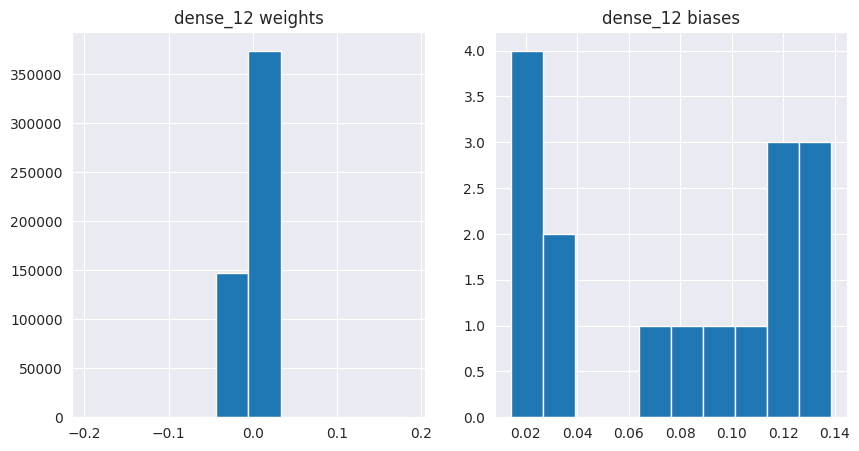
\includegraphics[width=1\textwidth]{cnn/CNN_Weight_Bias1.png}
  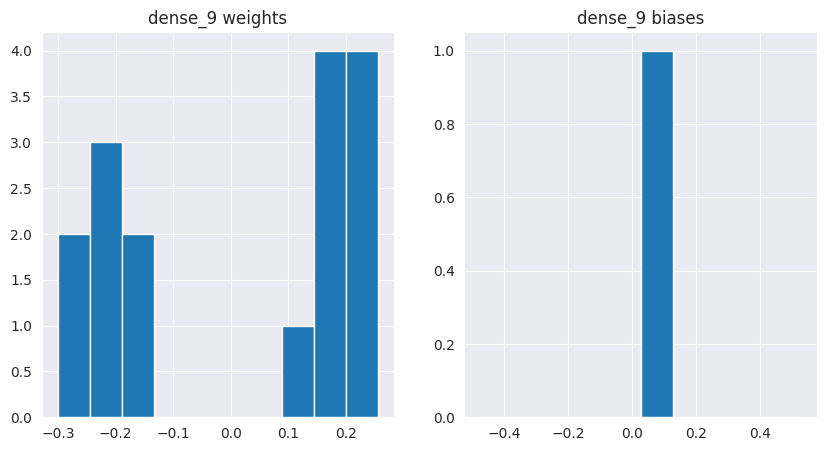
\includegraphics[width=1\textwidth]{cnn/CNN_Weight_Bias2.png}
  \caption{CNN Weights and Biases Evaluation}\label{fig:cnn_weight_bias}
\end{figure}

% help check pl0x - jwisgay %
% ben ben help check pl0x too %
The histograms show the distributions of weights and biases for the dense\_12 and dense\_13 layers in a CNN, indicating how the network's parameters have adapted through training. In the dense\_12 layer, the concentration of weights around zero suggests that many neurons may not be contributing effectively to the network's predictions, pointing to potential over-parameterization. The biases for this layer display a bimodal distribution, hinting at a variation in neuron activation thresholds. 
For the dense\_13 layer, a more dispersed weight distribution implies a differentiation in connection significance, with neurons possibly specialized for distinct patterns. The biases are skewed towards higher values, suggesting a propensity for neuron activation. 


\begin{figure}[H] 
  \centering
  \includegraphics[width=1\textwidth]{cnn/CNN_ROC.png}
  \caption{CNN ROC Curve Evaluation}\label{fig:cnn_roc_curve}
\end{figure}

% help check pl0x - jwisgay %
% ben ben help check pl0x too %
The CNN's ROC curve without DFT preprocessing demonstrates a high level of classification accuracy, as evidenced by an AUC of 0.93. This suggests that even without the frequency domain features provided by DFT, the CNN can effectively discriminate between the classes, with a low rate of false positives relative to true positives. The strong performance highlighted by the ROC curve indicates that the model is robust and can reliably make predictions in its current configuration.

\subsection{Convolution Neural Network With DFT \acrshort{cir} Data}\label{cnn_visual_dft}

\begin{figure}[H] 
  \centering
  \includegraphics[width=0.5\textwidth]{cnn/DFT/CNN_Confusion_Matrix.png}
  \caption{CNN Confusion Matrix (DFT)}\label{fig:cnn_confusion_matrix_dft}
\end{figure}

% help check pl0x - jwisgay %
% ben ben help check pl0x too %
The model has demonstrated commendable predictive strength, correctly identifying 3864 instances as the negative class (True Negatives) and 3594 as the positive class (True Positives). However, there are 328 occurrences where the model incorrectly predicted the positive class (False Positives), and 614 instances of misclassifying the positive class as negative (False Negatives). These inaccuracies indicate opportunities for model optimization. The metrics derived from the matrix accuracy, precision, recall, and F1 score serves as a statistical summary of the model's current performance, with an implication that the CNN, while proficient, could benefit from enhancements to reduce the number of false classifications and thus improve its overall predictive accuracy.

\begin{figure}[H] 
  \centering
  \includegraphics[width=0.5\textwidth]{cnn/DFT/CNN_Learning_Curve.png}
  \caption{CNN Learning Curve (DFT)}\label{fig:cnn_learning_curve_dft}
\end{figure}

% help check pl0x - jwisgay %
% ben ben help check pl0x too %
This learning curve for a DFT-processed CNN illustrates a rapid and effective learning process, with both training and validation accuracy rates plateauing at high levels, signifying proficient generalization. The corresponding losses decline swiftly, showing significant early improvements that taper off, indicating that the model has reached its learning capacity. The close alignment of the validation loss with the training loss throughout the training process suggests the model is well-tuned to the data, providing a good balance between learning the training data and maintaining performance on unseen data. The DFT preprocessing likely contributes to the model’s ability to extract relevant features for classification tasks, reinforcing its predictive power.
% maybe last sentence don need?? -jovian @any1 %

\begin{figure}[H] 
  \centering
  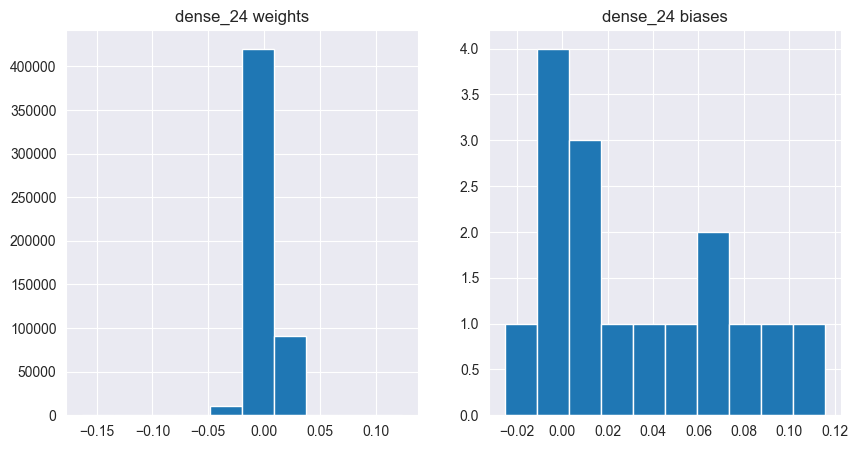
\includegraphics[width=0.4\textwidth]{cnn/DFT/CNN_Dense_Weights_1.png}
  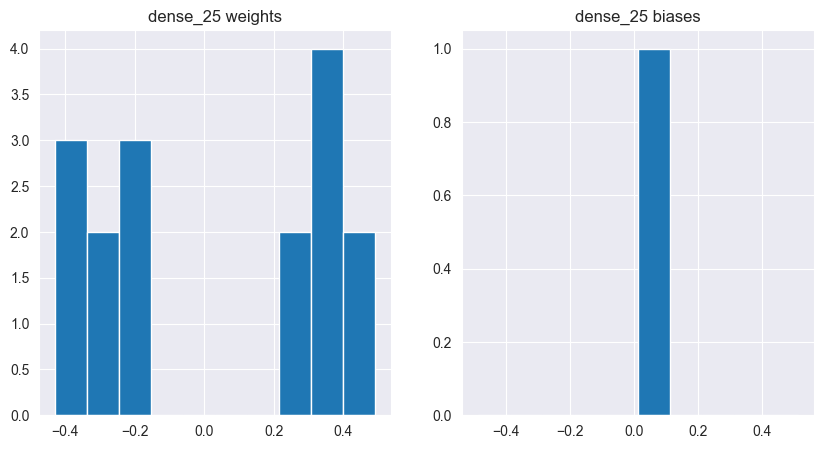
\includegraphics[width=0.4\textwidth]{cnn/DFT/CNN_Dense_Weights_2.png}
  \caption{CNN Weights and Biases Evaluation (DFT}\label{fig:cnn_weight_bias_dft}
\end{figure}

% help check pl0x - jwisgay %
% ben ben help check pl0x too %
The weight and bias histograms for the dense\_24 and dense\_25 layers of a DFT-trained CNN reveal distinct aspects of the network's learning dynamics. The dense\_24 layer's weights predominantly cluster around zero, hinting at potential inactivity or redundancy, possibly indicating an underutilized capacity for learning from the DFT-processed inputs. In contrast, the bias distribution in the same layer suggests neurons are calibrated with varied activation thresholds, allowing for differential responses to DFT features. The dense\_25 layer exhibits a broader spread of weight values, suggesting a richer engagement with the data and a more complex assimilation of features. Similarly, the biases in this layer tend to be positive, hinting at a uniformly higher neuron activation level, which may enhance the network's pattern recognition ability within the DFT-modified data landscape. These patterns underscore the nuanced interactions within the CNN's layers, potentially informing subsequent optimization and training strategies.

\begin{figure}[H] 
  \centering
  \includegraphics[width=0.5\textwidth]{cnn/DFT/CNN_ROC.png}
  \caption{CNN ROC Curve Evaluation (DFT)}\label{fig:cnn_roc_curve_dft}
\end{figure}

% help check pl0x - jwisgay %
% ben ben help check pl0x too %
The ROC curve derived from the DFT-processed data highlights the CNN's high discriminatory power, with an AUC of 0.95, reflecting its strong capability in distinguishing between the positive and negative classes. This high AUC value confirms the efficacy of the CNN, implying that the DFT preprocessing likely contributed positively to the model's classification performance. The curve's proximity to the ideal point indicates excellent sensitivity and specificity, confirming that the CNN, equipped with DFT, is a robust tool for making accurate predictions in this context.


%%%%%%%%%%%%%%%%%%%%%%%%%%%%%%%%%%%%%%%%%%%%%%%%%
% MLP Visualisation
%%%%%%%%%%%%%%%%%%%%%%%%%%%%%%%%%%%%%%%%%%%%%%%%%

% Send help jovian, fking die bodoh %
\subsection{Multilayer Perceptron}\label{mlp_visual}

\begin{figure}[H] 
  \centering
  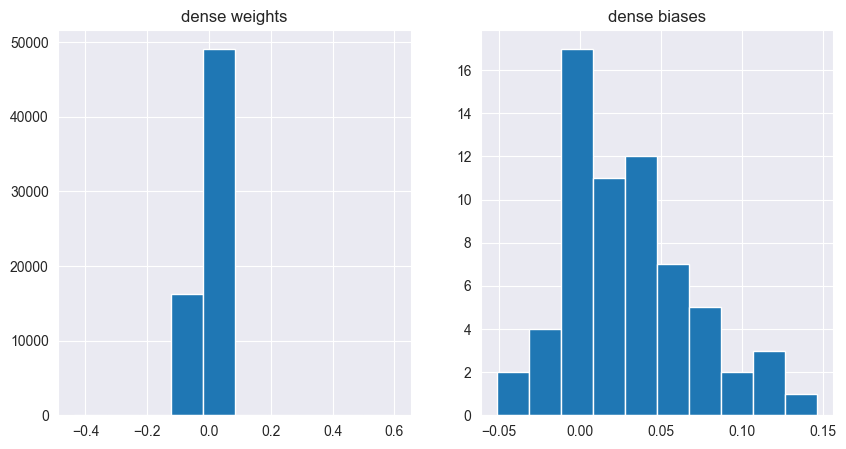
\includegraphics[width=1\textwidth]{mlp/Mlp_dense_biases.png}
  \caption{MLP Weights and Biases Evaluation}\label{fig:mlp_weights_biases}
\end{figure}

\begin{figure}[H] 
  \centering
  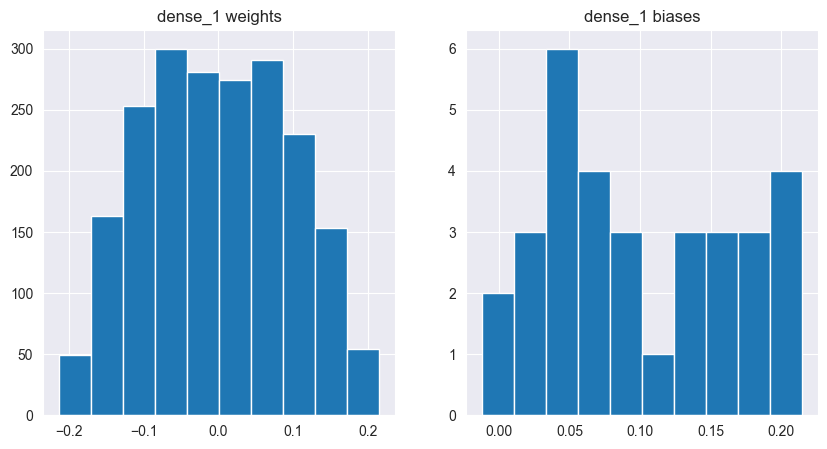
\includegraphics[width=1\textwidth]{mlp/Mlp_dense1_bias1.png}
  \caption{MLP Weights and Biases Evaluation}\label{fig:dense1_bias1}
\end{figure}

\begin{figure}[H] 
  \centering
  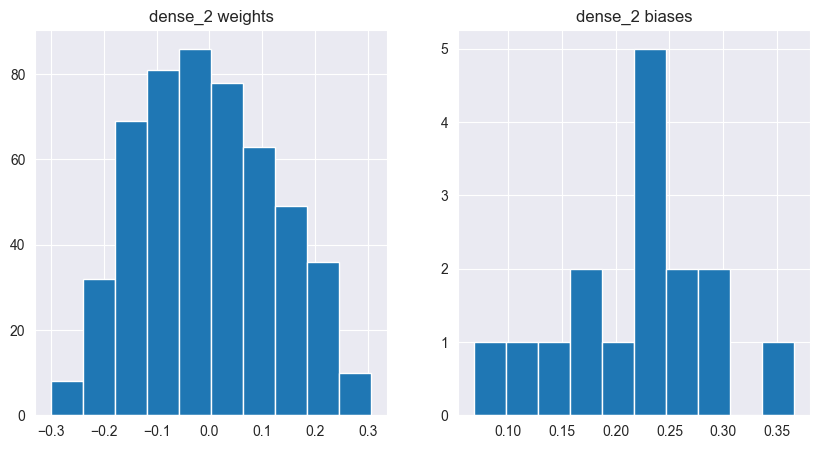
\includegraphics[width=1\textwidth]{mlp/Mlp_dense2_bias2.png}
  \caption{MLP Weights and Biases Evaluation}\label{fig:dense2_bias2}
\end{figure}

\begin{figure}[H] 
  \centering
  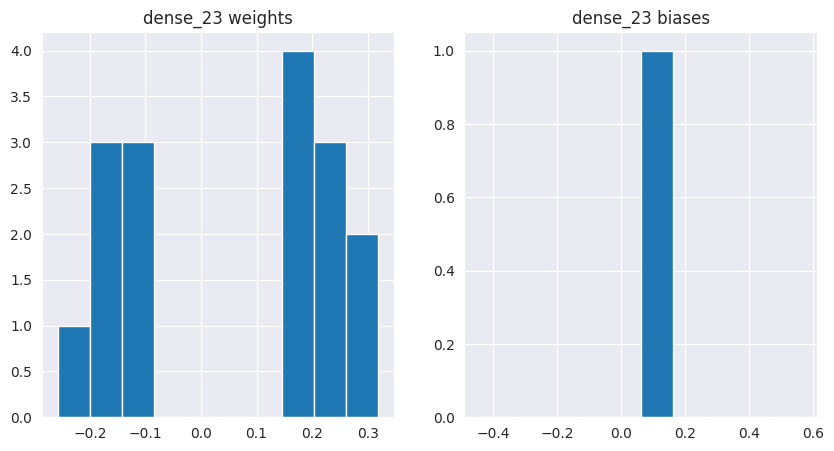
\includegraphics[width=1\textwidth]{mlp/Mlp_dense3_bias3.png}
  \caption{MLP Weights and Biases Evaluation}\label{fig:dense3_bias3}
\end{figure}

The weights and biases of the MLP model layers were visualized to understand their distributions. The weights in all layers (\texttt{dense\_20}, \texttt{dense\_21}, \texttt{dense\_22}, and \texttt{dense\_23}) are not close to zero, indicating they are likely being updated during training and contributing to the model’s learning. The weight distributions show a spread around zero, suggesting the model is capturing complex relationships in the data.

The biases in \texttt{dense\_20} and \texttt{dense\_22} introduce a slight positive bias to the activations in subsequent layers, potentially affecting the model’s predictions. The biases in \texttt{dense\_21} and \texttt{dense\_23} are centered around zero, with a slight spread towards positive values, introducing a small positive shift in the activations of the next layer. Overall, the model’s weights and biases suggest that it is learning effectively from the training data.


\begin{figure}[H] 
  \centering
  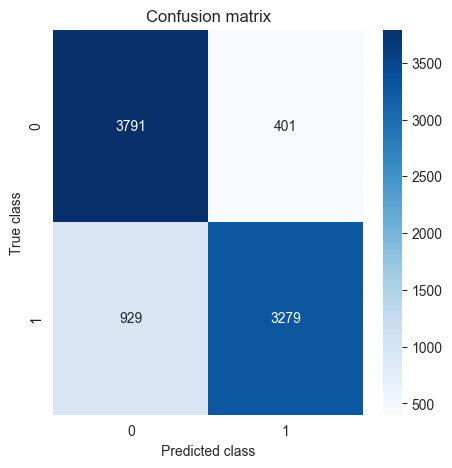
\includegraphics[width=1\textwidth]{mlp/Mlp_confusion_matrix.png}
  \caption{MLP Confusion Matrix}\label{fig:mpl_confusion_matrix}
\end{figure}

The MLP model performs admirably in categorizing NLOS/LOS signals, accurately identifying 3791 LOS signals (True Positives) and 3279 NLOS signals (True Negatives). However, it erroneously categorizes 401 NLOS signals as LOS (False Positives) and 929 LOS signals as NLOS (False Negatives). Although the model achieves a high overall accuracy by correctly classifying a considerable number of samples, the asymmetry in errors, particularly the higher number of False Negatives for LOS signals, suggests areas for improvement. This discrepancy may stem from the broader range of variations present in LOS signals compared to NLOS signals, indicating the need for further refinement to enhance the model's accuracy and balance in classification.

\begin{figure}[H] 
  \centering
  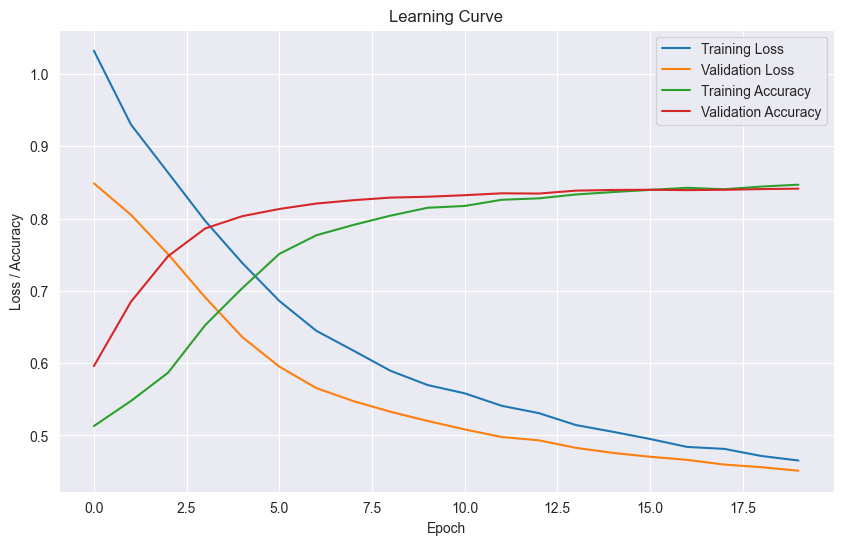
\includegraphics[width=1\textwidth]{mlp/Mlp_learning_curve.png}
  \caption{MLP Learning Curve}\label{fig:mlp_learning_curve}
\end{figure}

Positive indicators observed from the mlp learning curve includes the steadily increasing training accuracy, indicating the model is effectively learning patterns in the NLOS/LOS signal data over the 20 epochs. The rising validation accuracy suggests the model is successfully generalizing these learned patterns to new, unseen data, thereby avoiding overfitting. Additionally, the relatively small gap between the training and validation curves further supports the notion of good generalization and minimal overfitting. However, there is potential for further improvement, as the validation curves show signs of plateauing around epoch 20, indicating the model may be nearing its optimal performance on the validation data.

\begin{figure}[H] 
  \centering
  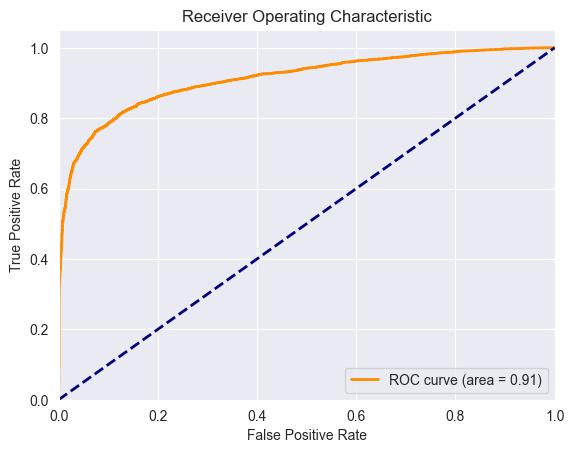
\includegraphics[width=1\textwidth]{mlp/Mlp_ROC_Curve.png}
  \caption{MLP ROC Curve Evaluation}\label{fig:mpl_roc_curve}
\end{figure}

The area under the ROC curve (AUC) is approximately 0.91, indicating strong model performance. The ROC curve illustrates the True Positive Rate (TPR) against the False Positive Rate (FPR) at different classification thresholds. The AUC signifies the probability of the model ranking a randomly selected positive instance (LOS) higher than a randomly selected negative instance (NLOS) across all thresholds, with 1 indicating perfect performance and 0.5 indicating chance performance.

The model's AUC of 0.91 suggests that the MLP model effectively distinguishes between NLOS and LOS signals, with a high likelihood of ranking true LOS signals higher than non-LOS signals and overall, this means that the MLP model is a strong classifier for NLOS/LOS signals.

% TODO jovian send help plox copy all 4 image into gpt4 %
\subsection{Multilayer Perceptron With DFT \acrshort{cir} Data}\label{mlp_visual_dft}

\begin{figure}[H] 
  \centering
  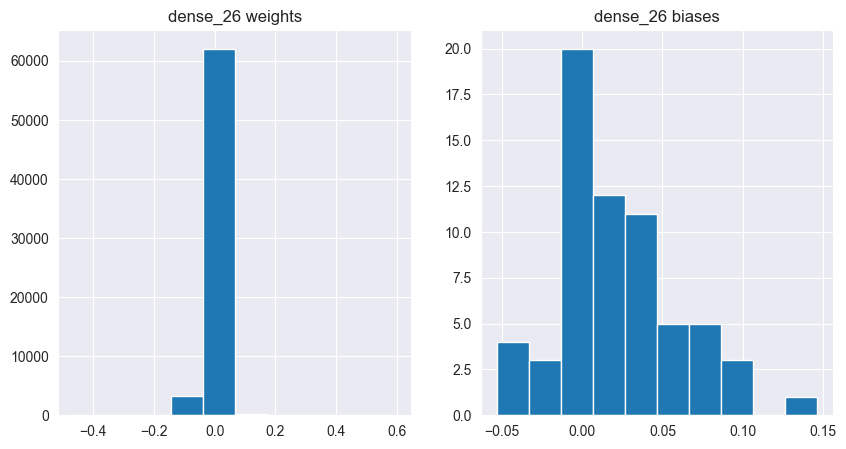
\includegraphics[width=1\textwidth]{mlp/Mlp_dense26_bias26_DFT.png}
  \caption{MLP Weights and Biases Evaluation DFT}\label{fig:Mlp_dense26_bias26_DFT}
\end{figure}

% help check pl0x - jwisgay %
% ben ben help check pl0x too %
The weight distribution is extremely concentrated around 0, with a huge spike near 0, and almost no weights of large magnitude. This could suggest that many neurons are not contributing much to the model's decisions, possibly due to dead neurons or because the model has not learned significant features from the data. The bias histogram also shows a concentration around a small positive value, which may indicate an adjustment to the activation levels of the neurons to fine-tune the output.

\begin{figure}[H] 
  \centering
  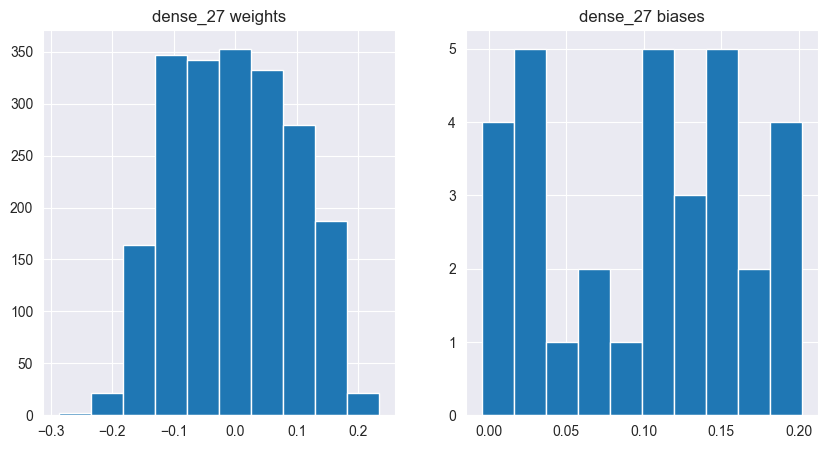
\includegraphics[width=1\textwidth]{mlp/Mlp_dense27_bias27_DFT.png}
  \caption{MLP Weights and Biases Evaluation DFT}\label{fig:Mlp_dense27_bias27_DFTMlp_dense27_bias27_DFT}
\end{figure}

% help check pl0x - jwisgay %
% ben ben help check pl0x too %
The weight distribution here is more spread out around 0, but still mostly centered within a narrow range. This could suggest that the neurons in this layer have learned a more diverse set of features from the DFT data, but the features are not highly distinct (as indicated by the close clustering around 0). The biases are somewhat evenly distributed across a range of positive values, which might suggest that the neurons in this layer are biased to be more active.


\begin{figure}[H] 
  \centering
  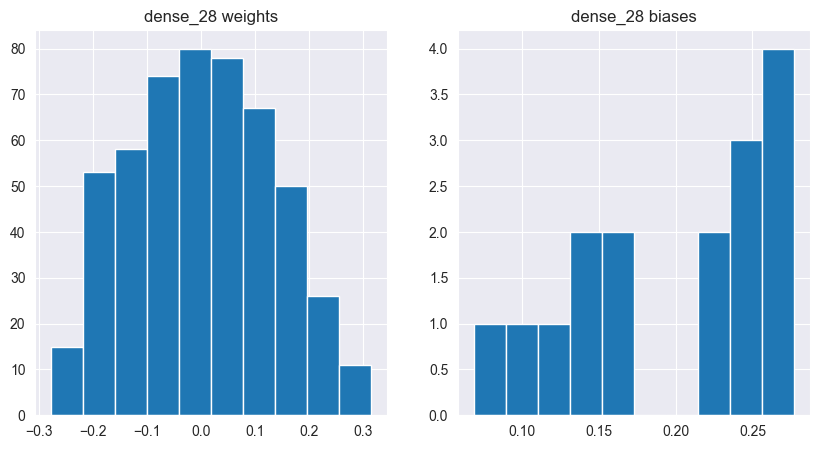
\includegraphics[width=1\textwidth]{mlp/Mlp_dense28_bias28_DFT.png}
  \caption{MLP Weights and Biases Evaluation DFT}\label{fig:Mlp_dense28_bias28_DFT}
\end{figure}

% help check pl0x - jwisgay %
% ben ben help check pl0x too %
The weights are again distributed around 0, with a slight skew towards positive values. This might imply that the layer is picking up on some features, but the asymmetry might also be a sign of the layer not utilizing its neurons uniformly. The biases here show a preference for higher positive values, indicating that the activation threshold for the neurons is being adjusted upward.

\begin{figure}[H] 
  \centering
  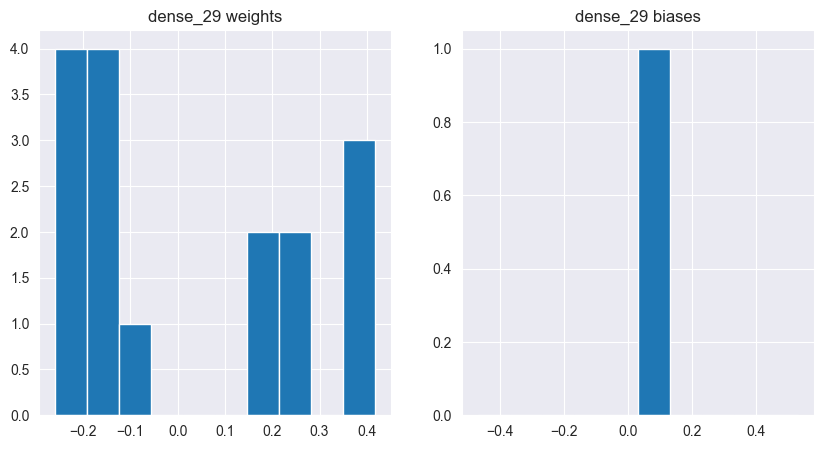
\includegraphics[width=1\textwidth]{mlp/Mlp_dense29_bias29_DFT.png}
  \caption{MLP Weights and Biases Evaluation DFT}\label{fig:Mlp_dense29_bias29_DFT}
\end{figure}

% help check pl0x - jwisgay %
% ben ben help check pl0x too %
The weights show a bi-modal distribution, with groupings at both negative and positive values and fewer weights near 0. This suggests that this layer's neurons are more actively engaged, possibly contributing to more complex feature detection. The bias distribution, heavily concentrated at a single positive value, might indicate a strong adjustment to the activation function, which could be a compensatory mechanism or a sign that the layer is trying to normalize the output in response to the DFT-processed inputs.

\begin{figure}[H] 
  \centering
  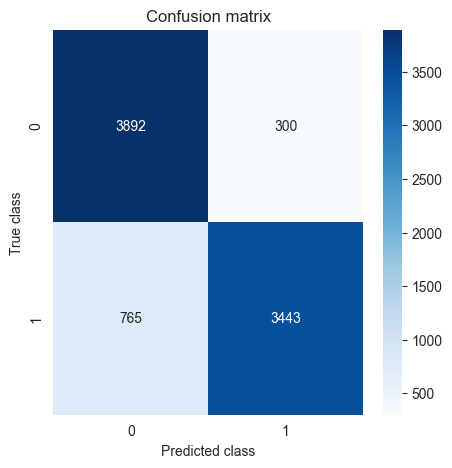
\includegraphics[width=1\textwidth]{mlp/Mlp_confusion_matrix_DFT.png}
  \caption{MLP Confusion Matrix DFT}\label{fig:Mlp_confusion_matrix_DFT}
\end{figure}

% help check pl0x - jwisgay %
% ben ben help check pl0x too - dk if this is what u want anot siaokia %
The confusion matrix provides a detailed portrayal of a Multi-Layer Perceptron (MLP) classifier's performance after training with Discrete Fourier Transform (DFT)-processed data for a binary classification task. It reveals that the MLP correctly predicted 3892 instances for class 0 and 3443 instances for class 1, designated as true negatives and true positives, respectively. However, the model also predicted 300 instances as class 1 that were actually class 0 (false positives) and missed 765 actual class 1 instances, classifying them as class 0 (false negatives). These results yield an accuracy of $\frac{(3443+3892)}{(3443+3892+300+765)}$, a precision of $\frac{3443}{(3443+300)}$ for class 1, and a recall of $\frac{3443}{3443+765}$ for the same. The F1 score, which harmonizes precision and recall, is particularly informative for the balance of false positives and false negatives. While the model demonstrates considerable accuracy, the presence of 765 false negatives warrants attention, as it could be critical in applications where failing to identify class 1 is costly. For an exhaustive assessment, these metrics should be viewed in conjunction with other performance measures like ROC and Precision-Recall curves, especially when dealing with imbalanced datasets or when the error costs are asymmetric.

\begin{figure}[H] 
  \centering
  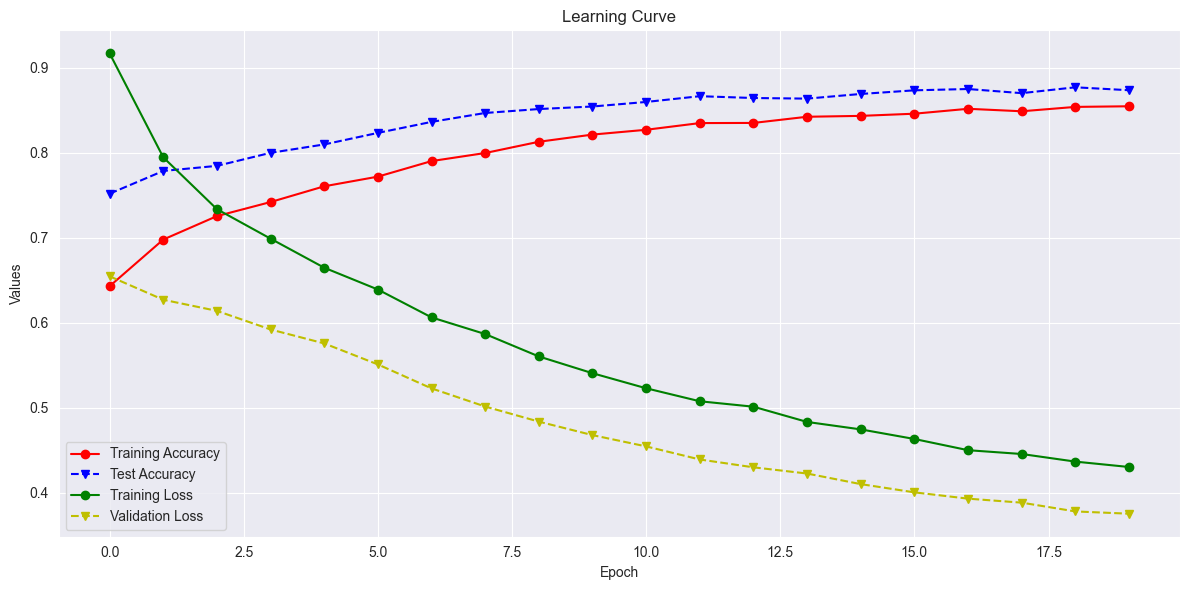
\includegraphics[width=1\textwidth]{mlp/Mlp_learning_curve_DFT.png}
  \caption{MLP Learning Curve DFT}\label{fig:Mlp_learning_curve_DFT}
\end{figure}

% help check pl0x - jwisgay %
% ben ben help check pl0x too %
Examining the learning curve of the MLP after training on DFT-processed data uncovers a familiar trend with notable differences. In this instance, there is a somewhat larger spread between the training and validation curves, hinting at a somewhat reduced capacity for generalization. Furthermore, the test and training accuracies have not quite met in the middle, which suggests the model may have room to further learn from the training data, and might see improvements with more training rounds or fine-tuning. Nonetheless, the model exhibits commendable performance metrics, with a final test loss standing at 37.5\%, an 87\% accuracy rate on the test set, and a ROC score reaching 94%.

\begin{figure}[H] 
  \centering
  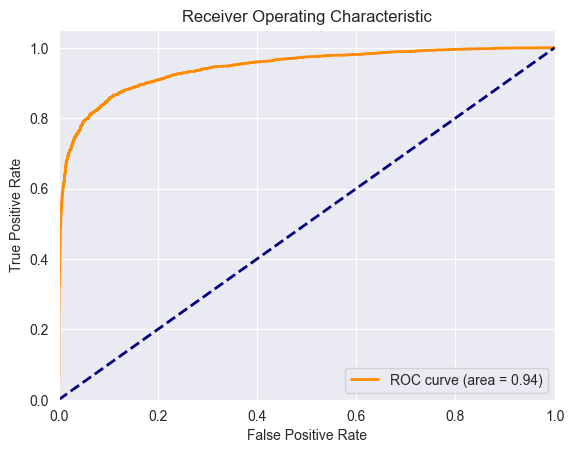
\includegraphics[width=1\textwidth]{mlp/Mlp_ROC_Curve_DFT.png}
  \caption{MLP ROC Curve Evaluation DFT}\label{fig:Mlp_ROC_Curve_DFT}
\end{figure}

% help check pl0x - jwisgay %
% ben ben help check pl0x too %
The ROC curve for the DFT-enhanced MLP model presents a robust indicator of the classifier's capability to distinguish between the binary classes. With the True Positive Rate on the y-axis and the False Positive Rate on the x-axis, the curve showcases the trade-offs between sensitivity and specificity across various thresholds. The AUC of 0.94 is significantly higher than the 0.5 baseline, which represents a random guess, underscoring the model's strong discriminative power. This high AUC value indicates a 94\% chance that the MLP will correctly rank a randomly chosen positive instance over a negative one, asserting the model's proficiency in classifying instances with a high degree of accuracy. In your report, emphasize that the MLP model, leveraging DFT-processed inputs, demonstrates an exceptional ability to differentiate between classes, making it a reliable tool for predictive tasks in your domain of application.
